\appendix
\chapter{Theory background}
\label{ch:theory}


This appendix describes the theory behind ConvNets and Recurrent Networks which is described along the Master Thesis for the sake of readability, since it is basic theory that is easy to find on books, online courses and blogs. We have left out of this material the basic theory on artificial neural networks and deep learning, which are deemed as minimum requirements for reading this thesis.

This chapter is almost entirely based on the book \textbf{Dive into Dive Learning (D2L)} \citep{Zhang2019d2l}, published online under a Creative Commons License (CC BY-NC-SA 4.0), with some modifications. In particular, we have excluded all the source code, rewritten some paragraphs to keep the consistence with the context, and added additional material to some parts that were of particular interest for our purposes.


\section{Convolutional Neural Networks}\label{sec:cnn}

As we have seen in the encoder-decoder architecture, the encoder used for image captioning is typically a Convolutional Neural Network (CNN). In this section we provide a brief explanation of this kind of network architecture and introduce some of the most remarkable examples, of which some have been used for the system developed in this project.

\subsection{From fully connected layers to convolutions}

2012 was the first year that neural nets grew to prominence as Alex Krizhevsky used them to win that year’s ImageNet Large Scale Visual Recognition Competition (ILSVRC) competition \citep{Krizhevsky2012}, with an astounding drop of the classification error record from 26\% to 15\%. Ever since then, a host of companies have been using deep learning at the core of their services, including Facebook (face recognition), Google (photo search, translation, voice recognition), Amazon (product recommendations), Pinterest (feed personalization), and Instagram (search infrastructure), amongst others.

Classical neural networks, as the Multi-Layer Perceptron (MLP), and fully connected architectures in general, were designed to work with tabular data, that is, data consisting of rows corresponding to examples and columns corresponding to features. With tabular data, we might anticipate that pattern we seek could require modeling interactions among the features, but do not assume anything a priori about which features are related to each other or in what way. In such cases, there is no way of exploiting such interactions when designing the network architecture, and MLPs are probably the best approach. However, once we start dealing with high-dimensional perceptual data, these "structure-less" networks can grow very unwieldy. 

For instance, let’s consider the task of classifying pictures into either cats or dogs. Say that we do a thorough job in data collection, collecting an annotated set of high-quality 1-megapixel photographs. This means that the input into a network has 1 million dimensions. Even an aggressive reduction to 1,000 hidden dimensions would require a dense (fully-connected) layer to support  $10^9$  parameters. Unless we have an extremely large dataset (perhaps billions?), lots of GPUs, a talent for extreme distributed optimization, and an extraordinary amount of patience, learning the parameters of this network may turn out to be impossible.

A careful reader might object to this argument on the basis that 1 megapixel resolution may not be necessary. However, while you could get away with 100,000 pixels, we grossly underestimated the number of hidden nodes that it typically takes to learn good hidden representations of images. Learning a binary classifier with so many parameters might seem to require that we collect an enormous dataset, perhaps comparable to the number of dogs and cats on the planet. And yet both humans and computers are able to distinguish cats from dogs quite well, seemingly contradicting these conclusions. That’s because images exhibit rich structure that is typically exploited by humans and machine learning models alike. For example, when perceiving images, the are two important properties that our visual systems use:

\begin{itemize}
    \item \textit{Translation invariance}: vision should respond similarly to the same object regardless of where it appears in the image.
    \item \textit{Locality}: for certain tasks our vision should focus on local regions, without regard for what else is happening in the image at greater distances.
\end{itemize}

Convolutional Neural Networks, or \textit{ConvNets}, for short, are a kind of artificial neural networks designed specifically to benefit  from these properties of the visual system. In fact, ConvNets were inspired by biological processes in that the connectivity pattern between neurons resembles the organization of the animal visual cortex. Individual cortical neurons respond to stimuli only in a restricted region of the visual field known as the receptive field. The receptive fields of different neurons partially overlap such that they cover the entire visual field.

ConvNets get their name from a mathematical operation called \textit{convolution}, although they actually correspond to a similar operation called \textit{cross-correlation}, represented by an asterisk within a circle, $\circledast$. ConvNets are built by stacking successive layers of units that apply two types of operation: convolutions (cross-correlation) and pooling. Now let us describe how these operations work in practice.

\subsection{Convolution layers}\label{subsec:conv_layers}

\subsubsection{The Cross-correlation operation}

The most important operation performed by ConvNets is the cross-correlation operation, often called \textit{convolution} operation, which takes an input array and a \textit{correlation kernel} array, and produce an output array through a \textit{cross-correlation operation}. Images are represented as 2D arrays of pixels, plus a third dimension when color channels are considered. But for the sake of simplicity, let's start with a 2D representation of images. 

\begin{figure}[hpt]
	\centering
	\includesvg{images/app/correlation.svg}
	\caption{Two dimensional cross-correlation operation. The shaded portions are the first output element and the input and kernel array elements used in its computation: $0 \times 0+1 \times 1+3 \times 2+4 \times 3=19$}
	\label{fig:correlation}
\end{figure}

In the two-dimensional cross-correlation operation (\cref{fig:correlation}), we begin with the convolution window positioned at the top-left corner of the input array and slide it across the input array, both from left to right and top to bottom. When the convolution window slides to a certain position, the input subarray contained in that window and the kernel array are multiplied (element-wise) and the resulting array is summed up yielding a single scalar value. This result is precisely the value of the output array at the corresponding location. Here, the output array has a height of 2 and width of 2 and the four elements are derived from the two-dimensional cross-correlation operation:

\begin{align*}
0 \times 0+1 \times 1+3 \times 2+4 \times 3=19,\\
1 \times 0+2 \times 1+4 \times 2+5 \times 3=25,\\
3 \times 0+4 \times 1+6 \times 2+7 \times 3=37,\\
4 \times 0+5 \times 1+7 \times 2+8 \times 3=43.
\end{align*}

Note that along each axis, the output array is slightly smaller than the input. Because the kernel has a width greater than one, and we can only computer the cross-correlation for locations where the kernel fits wholly within the image, the output size is given by the input size $H \times W$  minus the size of the kernel $h \times w$ via $(H-h+1)\times(W-w+1)$. This is the case since we need enough space to \textit{shift} the kernel across the image.

A convolutional layer cross-correlates (\textit{convolves}) the input and kernels and adds a scalar bias $b$ to produce an output. The parameters of the convolutional layer are precisely the values that constitute the kernel and the scalar bias. When training the models based on convolutional layers, we typically initialize the kernels randomly, just as we would with a fully-connected layer. Optionally, a convolutional layer may also apply an activation function $g$ to produce its final output, although we will not explain it here, since it is the same as for a fully connected layer.

Correlation kernels can be seen as feature detectors; for example, they can be used to detect edges in different orientations, such as vertical lines, horizontal lines, or curves of any shape. Designing an edge detector by finite differences $[1, -1]$ is neat if we know this is precisely what we are looking for. However, as we look at larger kernels, and consider successive layers of convolutions, it might be impossible to specify precisely what each filter should be doing manually. Fortunately, we do not need to define kernels by hand, since they can be learned automatically using backpropagation, as the weights of a fully connected layer.

\begin{figure}[hpt]
	\centering
	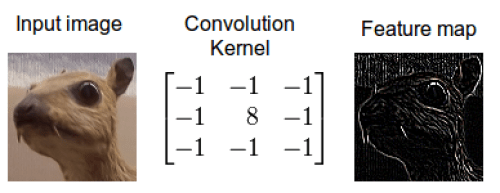
\includegraphics[scale=0.5]{images/app/edge-detection.png}
	\caption{Example of a convolution kernel for edge detection}
	\label{fig:edge-detection}
\end{figure}

\subsubsection{Padding}

In the previous example, our input had a height and width of 3 and a convolution kernel with a height and width of 2, yielding an output with a height and a width of 2. In general, assuming the input shape is  $n_h \times n_w$  and the convolution kernel window shape is $k_h \times k_w$, then the output shape will be

$$(n_h-k_h+1) \times (n_w-k_w+1)$$
 
Therefore, the output shape of the convolutional layer is determined by the shape of the input and the shape of the convolution kernel window.

In several cases we might want to incorporate particular techniques --padding and stride-- regarding the size of the output:
\begin{itemize}
    \item In general, since kernels generally have width and height greater than 1, that means that after applying many successive convolutions, we will wind up with an output that is much smaller than our input. If we start with a $240\times240$ pixel image, 10 layers of $5\times5$ convolutions reduce the image to $200\times200$ pixels, slicing off 30\% of the image and with it obliterating any interesting information on the boundaries of the original image. Padding handles this issue.
    \item In some cases, we want to reduce the resolution drastically if say we find our original input resolution to be unwieldy. Strides can help in these instances.
\end{itemize}

\begin{figure}[hpt]
	\centering
	\includesvg{images/app/conv_pad.svg}
	\caption{Two-dimensional cross-correlation with padding. The shaded portions are the input and kernel array elements used by the first output element: $0\times0+0\times1+0\times2+0\times3=0$}
	\label{fig:conv_pad}
\end{figure}

In general, if we add a total of  $p_h$  rows of padding (roughly half on top and half on bottom) and a total of  $p_w$  columns of padding (roughly half on the left and half on the right), the output shape will be

$$(n_h-k_h+p_h+1)\times(n_w-k_w+p_w+1)$$
 
This means that the height and width of the output will increase by  $p_h$  and  $p_w$  respectively.

In many cases, we will want to set  $p_h=k_h-1$  and  $p_w=k_w-1$  to give the input and output the same height and width. This will make it easier to predict the output shape of each layer when constructing the network. Assuming that  $k_h$  is odd here, we will pad  $p_h/2$ rows on both sides of the height. If $k_h$  is even, one possibility is to pad  $\lceil p_h/2\rceil$  rows on the top of the input and  $\lfloor p_h/2\rfloor$  rows on the bottom. We will pad both sides of the width in the same way.

ConvNets commonly use correlation kernels with odd height and width values, such as 1, 3, 5, or 7. Choosing odd kernel sizes has the benefit that we can preserve the spatial dimensionality while padding with the same number of rows on top and bottom, and the same number of columns on left and right.

Moreover, this practice of using odd kernels and padding to precisely preserve dimensionality offers a clerical benefit. For any two-dimensional array $X$, when the kernels size is odd and the number of padding rows and columns on all sides are the same, producing an output with the same height and width as the input, we know that the output $Y[i,j]$ is calculated by cross-correlation of the input and convolution kernel with the window centered on $X[i,j]$.

\subsubsection{Stride}

When computing the cross-correlation, we start with the convolution window at the top-left corner of the input array, and then slide it over all locations both down and to the right. In previous examples, we default to sliding one pixel at a time. However, sometimes, either for computational efficiency or because we wish to downsample, we move our window more than one pixel at a time, skipping the intermediate locations.

We refer to the number of rows and columns traversed per slide as the stride. So far, we have used strides of 1, both for height and width. Sometimes, we may want to use a larger stride. \cref{fig:conv_stride} shows a two-dimensional cross-correlation operation with a stride of 3 vertically and 2 horizontally. We can see that when the second element of the first column is output, the convolution window slides down three rows. The convolution window slides two columns to the right when the second element of the first row is output. When the convolution window slides two columns to the right on the input, there is no output because the input element cannot fill the window (unless we add padding).

\begin{figure}[hpt]
	\centering
	\includesvg{images/app/conv_stride.svg}
	\caption{Cross-correlation with strides of 3 and 2 for height and width respectively. The shaded portions are the output element and the input and core array elements used in its computation: $0\times0+0\times1+1\times2+2\times3=8,  0\times0+6\times1+0\times2+0\times3=6$}
	\label{fig:conv_stride}
\end{figure}

In general, when the stride for the height is $s_h$  and the stride for the width is $s_w$ , the output shape is

$$\lfloor(n_h-k_h+p_h+s_h)/s_h\rfloor \times \lfloor(n_w-k_w+p_w+s_w)/s_w\rfloor$$
 
If we set $p_h=k_h-1$  and  $p_w=k_w-1$ , then the output shape will be simplified to $\lfloor(n_h+s_h-1)/s_h\rfloor \times \lfloor(n_w+s_w-1)/s_w\rfloor$. Going a step further, if the input height and width are divisible by the strides on the height and width, then the output shape will be $(n_h/s_h)\times(n_w/s_w)$.

For the sake of brevity, when the padding number on both sides of the input height and width are $p_h$  and $p_w$  respectively, we call the padding $(p_h,p_w)$. Specifically, when  $p_h=p_w=p$, the padding is $p$. When the strides on the height and width are $s_h$ and $s_w$, respectively, we call the stride $(s_h,s_w)$. Specifically, when $s_h=s_w=s$, the stride is $s$. By default, the padding is 0 and the stride is 1. In practice we rarely use inhomogeneous strides or padding, i.e., we usually have $p_h=p_w$ and $s_h=s_w$.

\subsubsection{Multiple Input and Output Channels}

While we have described the multiple channels that comprise each image (e.g. color images have the standard RGB channels to indicate the amount of red, green and blue), until now, we simplified all of our numerical examples by working with just a single input and a single output channel. This has allowed us to think of our inputs, convolutional kernels, and outputs each as two-dimensional arrays.

When we add channels into the mix, our inputs and hidden representations both become three-dimensional arrays. For example, each RGB input image has shape $3\times h\times w$. We refer to this axis, with a size of 3, as the channel dimension. In this section, we will take a deeper look at convolution kernels with multiple input and multiple output channels.

\paragraph{Multiple Input Channels}

When the input data contains multiple channels, we need to construct a convolution kernel with the same number of input channels as the input data, so that it can perform cross-correlation with the input data. Assuming that the number of channels for the input data is $c_i$, the number of input channels of the convolution kernel also needs to be $c_i$. If our convolution kernel’s window shape is $k_h\times k_w$, then when $c_i=1$, we can think of our convolution kernel as just a two-dimensional array of shape $k_h\times k_w$.

However, when $c_i>1$, we need a kernel that contains an array of shape $k_h\times k_w$ for each input channel. Concatenating these $c_i$ arrays together yields a convolution kernel of shape $c_i\times k_h\times k_w$. Since the input and convolution kernel each have $c_i$ channels, we can perform a cross-correlation operation on the two-dimensional array of the input and the two-dimensional kernel array of the convolution kernel for each channel, adding the $c_i$ results together (summing over the channels) to yield a two-dimensional array. This is the result of a two-dimensional cross-correlation between multi-channel input data and a multi-input channel convolution kernel.

\cref{fig:conv_multi_in} shows an example of a 2D cross-correlation with two input channels. 

\begin{figure}[hpt]
	\centering
	\includesvg{images/app/conv_multi_in.svg}
	\caption{Cross-correlation computation with 2 input channels. The shaded portions are the first output element as well as the input and kernel array elements used in its computation:  $(1 \times 1+2 \times 2+4\times3+5\times4)+(0\times0+1 \times 1+3\times2+4\times3)=56.$}
	\label{fig:conv_multi_in}
\end{figure}

\paragraph{Multiple Output Channels}

Regardless of the number of input channels, so far we always ended up with one output channel. However, as we discussed earlier, it turns out to be essential to have multiple channels at each layer. In the most popular neural network architectures, we actually increase the channel dimension as we go higher up in the neural network, typically downsampling to trade off spatial resolution for greater channel depth. Intuitively, you could think of each channel as responding to some different set of features. Reality is a bit more complicated than the most naive intepretations of this intuition since representations are not learned independently but are rather optimized to be jointly useful. So it may not be that a single channel learns an edge detector but rather that some direction in channel space corresponds to detecting edges.

Denote by $c_i$ and $c_o$  the number of input and output channels, respectively, and let $k_h$ and $k_w$ be the height and width of the kernel. To get an output with multiple channels, we can create a kernel array of shape $c_i \times k_h \times k_w$ for each output channel. We concatenate them on the output channel dimension, so that the shape of the convolution kernel is $c_o \times c_i \times k_h \times k_w$. In cross-correlation operations, the result on each output channel is calculated from the convolution kernel corresponding to that output channel and takes input from all channels in the input array.

\paragraph{1 x 1 convolutional layers}

At first, a $1 \times 1$  convolution, i.e.  $k_h=k_w=1$, does not seem to make much sense. After all, a convolution correlates adjacent pixels. A $1 \times 1$ convolution obviously does not. Nonetheless, they are popular operations that are sometimes included in the designs of complex deep networks. Let’s see in some detail what it actually does.

Because the minimum window is used, the $1 \times 1$ convolution loses the ability of larger convolutional layers to recognize patterns consisting of interactions among adjacent elements in the height and width dimensions. The only computation of the $1 \times 1$ convolution occurs on the channel dimension.

\cref{fig:conv_1x1} shows the cross-correlation computation using the $1 \times 1$ convolution kernel with 3 input channels and 2 output channels. Note that the inputs and outputs have the same height and width. Each element in the output is derived from a linear combination of elements at the same position in the input image. You could think of the $1 \times 1$  convolutional layer as constituting a fully-connected layer applied at every single pixel location to transform the $c_i$ corresponding input values into $c_o$ output values. Because this is still a convolutional layer, the weights are tied across pixel location Thus the $1 \times 1$  convolutional layer requires $c_o \times c_i$ weights (plus the bias terms).

\begin{figure}[hpt]
	\centering
	\includesvg{images/app/conv_1x1.svg}
	\caption{Cross-correlation computation using a $1 \times 1$ convolution kernel with 3 input channels and 2 output channels. The inputs and outputs have the same height and width.}
	\label{fig:conv_1x1}
\end{figure}

\subsection{Pooling layers}\label{subsec:pool_layers}

Often, as we process images, we want to gradually reduce the spatial resolution of our hidden representations, aggregating information so that the higher up we go in the network, the larger the receptive field (in the input) to which each hidden node is sensitive.

Often our ultimate task asks some global question about the image, e.g., does it contain a cat? So typically the nodes of our final layer should be sensitive to the entire input. By gradually aggregating information, yielding coarser and coarser maps, we accomplish this goal of ultimately learning a global representation, while keeping all of the advantages of convolutional layers at the intermediate layers of processing.

Moreover, when detecting lower-level features, such as edges, we often want our representations to be somewhat invariant to translation. For instance, if we take the image $X$ with a sharp delineation between black and white and shift the whole image by one pixel to the right, i.e. $Z[i,j] = X[i,j+1]$ then the output for the new image $Z$ might be vastly different. The edge will have shifted by one pixel and with it all the activations. In reality, objects hardly ever occur exactly at the same place. In fact, even with a tripod and a stationary object, vibration of the camera due to the movement of the shutter might shift everything by a pixel or so.

Pooling layers serve the dual purpose of mitigating the sensitivity of convolutional layers to location and of spatially downsampling representations.

\subsubsection{Maximum Pooling and Average Pooling}

Like convolutional layers, pooling layers apply a fixed-shape window that slides over all regions in the input according to its stride, computing a single output for each location traversed by the fixed-shape window (sometimes known as the pooling window). However, unlike convolutional layers, which need parameters to represent the correlation kernels, the pooling layer contains no parameters (there is no kernel). Instead, pooling operators are deterministic, typically calculating either the maximum or the average value of the elements in the pooling window. These operations are called maximum pooling (\textit{max pooling} for short) and \textit{average pooling}, respectively.

In both cases, as with the cross-correlation operator, we can think of the pooling window as starting from the top left of the input array and sliding across the input array from left to right and top to bottom. At each location that the pooling window hits, it computes the maximum or average value of the input subarray in the window (depending on whether max or average pooling is employed).

\begin{figure}[hpt]
	\centering
	\includesvg{images/app/pooling.svg}
	\caption{Maximum pooling with a pooling window shape of $2\times2$. The shaded portions represent the first output element and the input element used for its computation:  $\max(0,1,3,4)=4$.}
	\label{fig:pooling}
\end{figure}

The output array in \cref{fig:pooling} has a height of 2 and a width of 2. The four elements are derived from the maximum value of $\text{max}$:

\begin{align*}
\max(0,1,3,4)=4,\\
\max(1,2,4,5)=5,\\
\max(3,4,6,7)=7,\\
\max(4,5,7,8)=8.\\
\end{align*}

A pooling layer with a pooling window shape of $p \times q$ is called a $p \times q$ pooling layer. The pooling operation is called $p \times q$ pooling.

Let us return to the object edge detection example mentioned at the beginning of this section. Now we will use the output of the convolutional layer as the input for $2 \times 2$  max pooling. Set the convolutional layer input as $X$ and the pooling layer output as $Y$. Whether or not the values of $X[i, j]$ and $X[i, j+1]$ are different, or $X[i, j+1]$ and $X[i, j+2]$ are different, the pooling layer outputs all include $Y[i, j]=1$. That is to say, using the $2 \times 2$ maximum pooling layer, we can still detect if the pattern recognized by the convolutional layer moves no more than one element in height and width.

\subsubsection{Padding and Stride}

As with convolutional layers, pooling layers can also change the output shape. And as before, we can alter the operation to achieve a desired output shape by padding the input and adjusting the stride.

When processing multi-channel input data, the pooling layer pools each input channel separately, rather than adding the inputs of each channel by channel as in a convolutional layer. This means that the number of output channels for the pooling layer is the same as the number of input channels

\subsubsection{Batch normalization}\label{subsubsec:batch-norm}

Training deep models is difficult and getting them to converge in a reasonable amount of time can be tricky. In this section, we describe batch normalization, one popular and effective technique that has been found to accelerate the convergence of deep nets and together with residual blocks, which we cover later has recently enabled practitioners  to routinely train networks with over 100 layers.

Let's review some of the practical challenges when training deep networks.

\begin{enumerate}
    \item Data preprocessing often proves to be a crucial consideration for effective statistical modeling. Standardizing input data typically makes it easier to train models since parameters are a-priori at a similar scale.
    \item For a typical MLP or CNN, as we train the model, the activations in intermediate layers of the network may assume different orders of magnitude (both across nodes in the same layer, and over time due to updating the model's parameters). The authors of the batch normalization technique postulated that this drift in the distribution of activations could hamper the convergence of the network. Intuitively, we might conjecture that if one layer has activation values that are 100x that of another layer, we might need to adjust learning rates adaptively per layer (or even per node within a layer).
    \item Deeper networks are complex and easily capable of overfitting. This means that regularization becomes more critical. Empirically, we note that even with dropout, models can overfit badly and we might benefit from other regularization heuristics.
\end{enumerate}

In 2015, \cite{Ioffe2015} introduced Batch Normalization (BN), a clever heuristic that has proved immensely useful for improving the reliability and speed of convergence when training deep models. In each training iteration, BN normalizes the activations of each hidden layer node (on each layer where it is applied) by subtracting its mean and dividing by its standard deviation, estimating both based on the current minibatch. Note that if our batch size was $1$,  we wouldn't be able to learn anything because during training, every hidden node would take value $0$. However, with large enough minibatches, the approach proves effective and stable.

In a nutshell, the idea in Batch Normalization is  to transform the activation at a given layer from $\mathbf{x}$ to

$$\mathrm{BN}(\mathbf{x}) = \mathbf{\gamma} \odot \frac{\mathbf{x} - \hat{\mathbf{\mu}}}{\hat\sigma} + \mathbf{\beta}$$

Here, $\hat{\mathbf{\mu}}$ is the estimate of the mean and $\hat{\mathbf{\sigma}}$ is the estimate of the variance. 
The result is that the activations are approximately rescaled to zero mean and unit variance. Since this may not be quite what we want, we allow for a coordinate-wise scaling coefficient $\mathbf{\gamma}$ and an offset $\mathbf{\beta}$. Consequently, the activations for intermediate layers cannot diverge any longer: we are actively rescaling them back to a given order of magnitude via $\mathbf{\mu}$ and $\sigma$. Intuitively, it is hoped that this normalization allows us to be more aggressive in picking large learning rates. To address the fact that in some cases the activations may actually \textit{need} to differ from standardized data, BN also introduces scaling coefficients $\mathbf{\gamma}$ and an offset $\mathbf{\beta}$.

In principle, we might want to use all of our training data to estimate the mean and variance. However, the activations corresponding to each example change each time we update our model. To remedy this problem, BN uses only the current minibatch for estimating $\hat{\mathbf{\mu}}$ and $\hat\sigma$. It is precisely due to this fact that we normalize based only on the \textit{current batch}
that \textit{batch normalization} derives its name. To indicate which minibatch $\mathcal{B}$ we draw this from, we denote the quantities with $\hat{\mathbf{\mu}}_\mathcal{B}$ and $\hat\sigma_\mathcal{B}$.

$$\hat{\mathbf{\mu}}_\mathcal{B} \leftarrow \frac{1}{|\mathcal{B}|} \sum_{\mathbf{x} \in \mathcal{B}} \mathbf{x}
\text{ and }
\hat{\mathbf{\sigma}}_\mathcal{B}^2 \leftarrow \frac{1}{|\mathcal{B}|} \sum_{\mathbf{x} \in \mathcal{B}} (\mathbf{x} - \mathbf{\mu}_{\mathcal{B}})^2 + \epsilon$$

Note that we add a small constant $\epsilon > 0$ to the variance estimate to ensure that we never end up dividing by zero, 
even in cases where the empirical variance estimate might vanish by accident. The estimates $\hat{\mathbf{\mu}}_\mathcal{B}$ 
and $\hat{\mathbf{\sigma}}_\mathcal{B}$ counteract the scaling issue by using unbiased but noisy estimates of mean and variance. 
Normally we would consider this a problem. After all, each minibatch has different data, different labels and with it, different activations, predictions and errors. As it turns out, this is actually beneficial. This natural variation appears to act as a form of regularization, conferring benefits (as observed empirically) in mitigating overfitting. 

In other recent preliminary research, \citet{Teye2018} and \citet{Luo2019} relate the properties of BN to Bayesian Priors and penalties respectively. 
In particular, this sheds some light on the puzzle why BN works best for moderate sizes of minibatches in the range 50-100.

We are now ready to take a look at how batch normalization works in practice.

\paragraph{Batch Normalization Layers}

The batch normalization methods for fully-connected layers and convolutional layers are slightly different. This is due to the dimensionality of the data 
generated by convolutional layers. We discuss both cases below. Note that one of the key differences between BN and other layers is that BN operates on a a full minibatch at a time (otherwise it cannot compute the mean and variance parameters per batch).

\paragraph{Fully-Connected Layers}

Usually we apply the batch normalization layer between the affine transformation and the activation function in a fully-connected layer. In the following, we denote by $\mathbf{u}$ the input and by $\mathbf{x} = \mathbf{W}\mathbf{u} + \mathbf{b}$ the output of the linear transform. This yields the following variant of BN:

$$\mathbf{y} = \phi(\mathrm{BN}(\mathbf{x})) =  \phi(\mathrm{BN}(\mathbf{W}\mathbf{u} + \mathbf{b}))$$

Recall that mean and variance are computed on the \textit{same} minibatch $\mathcal{B}$ on which the transformation is applied. Also recall that the scaling coefficient $\mathbf{\gamma}$ and the offset $\mathbf{\beta}$ are parameters that need to be learned. They ensure that the effect of batch normalization can be neutralized as needed.

\paragraph{Convolutional Layers}

For convolutional layers, batch normalization occurs after the convolution computation and before the application of the activation function. 
If the convolution computation outputs multiple channels, we need to carry out batch normalization for \textit{each} of the outputs of these channels, 
and each channel has an independent scale parameter and shift parameter, both of which are scalars. Assume that there are $m$ examples in the mini-batch. 
On a single channel, we assume that the height and width of the convolution computation output are $p$ and $q$, respectively. We need to carry out batch normalization for $m \times p \times q$ elements in this channel simultaneously. While carrying out the standardization computation for these elements, 
we use the same mean and variance. In other words, we use the means and variances of the $m \times p \times q$ elements in this channel rather than one per pixel.

\paragraph{Batch Normalization During Prediction}

At prediction time, we might not have the luxury of computing offsets per batch—we might be required to make one prediction at a time. Secondly, the uncertainty in $\mathbf{\mu}$ and $\mathbf{\sigma}$, as arising from a minibatch are undesirable once we've trained the model. One way to mitigate this is to compute more stable estimates on a larger set for once (e.g. via a moving average) and then fix them at prediction time. Consequently, BN behaves differently during training and at test time (recall that dropout also behaves differently at train and test times).

% \subsection{Examples of concrete CNN architectures}

% \subsubsection{Classical convolutional networks: LeNet}

% In this section, we will introduce one of the first published convolutional neural networks whose benefit was first demonstrated by  \citet{Lecun1998}, for the purpose of recognizing handwritten digits in images. In the 90s, their experiments with \href{http://yann.lecun.com/exdb/lenet/}{LeNet} gave the first compelling evidence that it was possible to train convolutional neural networks by backpropagation. Their model achieved outstanding results at the time (only matched by Support Vector Machines at the time) and was adopted to recognize digits for processing deposits in ATM machines. Some ATMs still runn the code that Yann and his colleague Leon Bottou wrote in the 1990s.

% In a rough sense, we can think LeNet as consisting of two parts: (i) a block of convolutional layers; and (ii) a block of fully-connected layers. Before getting into the weeds, let’s briefly review the model in \cref{fig:lenet}

% \begin{figure}[hpt]
% 	\centering
% 	\includesvg[scale=0.4]{images/app/lenet.svg}
% 	\caption{Data flow in LeNet 5. The input is a handwritten digit, the output a probabilitiy over 10 possible outcomes.}
% 	\label{fig:lenet}
% \end{figure}

% The basic units in the convolutional block are a convolutional layer and a subsequent average pooling layer (note that max-pooling works better, but it had not been invented in the 90s yet). The convolutional layer is used to recognize the spatial patterns in the image, such as lines and the parts of objects, and the subsequent average pooling layer is used to reduce the dimensionality. The convolutional layer block is composed of repeated stacks of these two basic units. Each convolutional layer uses a $5 \times 5$  kernel and processes each output with a \textit{sigmoid} activation function (again, note that \textit{ReLU}s are now known to work more reliably, but had not been invented yet). The first convolutional layer has 6 output channels, and second convolutional layer increases channel depth further to 16.

% However, coinciding with this increase in the number of channels, the height and width are shrunk considerably. Therefore, increasing the number of output channels makes the parameter sizes of the two convolutional layers similar. The two average pooling layers are of size  $2 \times 2$  and take stride 2 (note that this means they are non-overlapping). In other words, the pooling layer downsamples the representation to be precisely one quarter the pre-pooling size.

% The convolutional block emits an output with size given by $(batch size, channel, height, width)$. Before we can pass the convolutional block’s output to the fully-connected block, we must flatten each example in the mini-batch. In other words, we take this 4D input and transform it into the 2D input expected by fully-connected layers: as a reminder, the first dimension indexes the examples in the mini-batch and the second gives the flat vector representation of each example. LeNet’s fully-connected layer block has three fully-connected layers, with 120, 84, and 10 outputs, respectively. Because we are still performing classification, the 10 dimensional output layer corresponds to the number of possible output classes.

% Note that the height and width of the representation at each layer throughout the convolutional block is reduced (compared to the previous layer). The convolutional layer uses a kernel with a height and width of 5, which with only  2  pixels of padding in the first convolutional layer and none in the second convolutional layer leads to reductions in both height and width by 2 and 4 pixels, respectively. Moreover each pooling layer halves the height and width. However, as we go up the stack of layers, the number of channels increases layer-over-layer from 1 in the input to 6 after the first convolutional layer and 16 after the second layer. Then, the fully-connected layer reduces dimensionality layer by layer, until emitting an output that matches the number of image classes.

% \cref{fig:lenet-vert} shows a diagram of LeNet5 architecture in a compressed format, the one we will use for the rest of this section.

% \begin{figure}[hpt]
% 	\centering
% 	\includesvg[scale=0.7]{images/app/lenet-vert.svg}
% 	\caption{Compressed notation for LeNet5}
% 	\label{fig:lenet-vert}
% \end{figure}


% \paragraph{Summary}

% \begin{itemize}
%     \item A convolutional neural network (in short, ConvNet) is a network using convolutional layers.
%     \item In a ConvNet we alternate between convolutions, nonlinearities and often also pooling operations.
%     \item Ultimately the resolution is reduced prior to emitting an output via one (or more) dense layers.
%     \item LeNet was the first successful deployment of such a network.
% \end{itemize}

% \subsubsection{Modern convolutional architectures}\label{subsubsec:modern_cnn}

% Although convolutional neural networks were well known in the computer vision and machine learning communities following the introduction of LeNet, they did not immediately dominate the field. Although LeNet achieved good results on early small data sets, the performance and feasibility of training convolutional networks on larger, more realistic datasets had yet to be established
% In fact, for much of the intervening time between the early 1990s and the watershed results of 2012, neural networks were often surpassed by other machine learning methods, such as support vector machines.

% A major breakthrough came when Alex Krizhevsky and Ilya Sutskever implemented a deep convolutional neural network that could run on GPU hardware. They realized that the computational bottlenecks in CNNs (convolutions and matrix multiplications) are all operations that could be parallelized in hardware. Using two NIVIDA GTX 580s with 3GB of memory, they implemented fast convolutions. The code \href{https://code.google.com/archive/p/cuda-convnet/}{cuda-convnet} was good enough that for several years it was the industry standard and powered the first couple years of the deep learning boom.

% \subsubsubsection{AlexNet: first large-scale ConvNet}

% AlexNet was introduced in 2012, named after Alex Krizhevsky, the first author of the breakthrough ImageNet classification paper \citep{Krizhevsky2012}. AlexNet, which employed an 8-layer convolutional neural network, won the ImageNet Large Scale Visual Recognition Challenge 2012 by a phenomenally large margin. This network proved, for the first time, that the features obtained by learning can transcend manually-design features, breaking the previous paradigm in computer vision. The architectures of AlexNet and LeNet are \textit{very similar}, as the diagram below illustrates. Note that we provide a slightly streamlined version of AlexNet removing some of the design quirks that were needed in 2012 to make the model fit on two small GPUs.

% \begin{figure}[hpt]
% 	\centering
% 	\includesvg[scale=0.8]{images/app/alexnet-all.svg}
% 	\caption{LeNet (left) and AlexNet (right)}
% 	\label{fig:alexnet}
% \end{figure}

% The design philosophies of AlexNet and LeNet are very similar, but there are also significant differences. First, AlexNet is much deeper than the comparatively small LeNet5. AlexNet consists of eight layers: five convolutional layers, two fully-connected hidden layers, and one fully-connected output layer. Second, AlexNet used the ReLU instead of the sigmoid as its activation function.

% \paragraph{Architecture}

% In AlexNet's first layer, the convolution window shape is $11\times11$. Since most images in ImageNet are more than ten times higher and wider than the MNIST images, objects in ImageNet data tend to occupy more pixels. Consequently, a larger convolution window is needed to capture the object. The convolution window shape in the second layer is reduced to $5\times5$, followed by $3\times3$. In addition, after the first, second, and fifth convolutional layers, the network adds maximum pooling layers with a window shape of $3\times3$ and a stride of 2. Moreover, AlexNet has ten times more convolution channels than LeNet.

% After the last convolutional layer are two fully-connected layers with 4096 outputs. These two huge fully-connected layers produce model parameters of nearly 1 GB. Due to the limited memory in early GPUs, the original AlexNet used a dual data stream design,
% so that each of their two GPUs could be responsible for storing and computing only its half of the model. Fortunately, GPU memory is comparatively abundant now, so we rarely need to break up models across GPUs these days.

% \paragraph{Activation functions}

% Second, AlexNet changed the sigmoid activation function to a simpler ReLU activation function. On the one hand, the computation of the ReLU activation function is simpler. For example, it does not have the exponentiation operation found in the sigmoid activation function. On the other hand, the ReLU activation function makes model training easier when using different parameter initialization methods. This is because, when the output of the sigmoid activation function is very close to 0 or 1, the gradient of these regions is almost 0, so that back propagation cannot continue to update some of the model parameters. In contrast, the gradient of the ReLU activation function in the positive interval is always 1. Therefore, if the model parameters are not properly initialized, the sigmoid function may obtain a gradient of almost 0 in the positive interval, so that the model cannot be effectively trained.

% \paragraph{Capacity Control and Preprocessing}

% AlexNet controls the model complexity of the fully-connected layer by dropout, while LeNet only uses weight decay. To augment the data even further, the training loop of AlexNet added a great deal of image augmentation, such as flipping, clipping, and color changes.
% This makes the model more robust and the larger sample size effectively reduces overfitting.

% \paragraph{Summary}

% \begin{itemize}
%     \item AlexNet has a similar structure to that of LeNet, but uses more convolutional layers and a larger parameter space to fit the large-scale data set ImageNet.
%     \item Today AlexNet has been surpassed by much more effective architectures but it is a key step from shallow to deep networks that are used nowadays.
%     \item Although it seems that there are only a few more lines in AlexNet's implementation than in LeNet, it took the academic community many years to embrace this conceptual change and take advantage of its excellent experimental results. This was also due to the lack of efficient computational tools.
%     \item Dropout, ReLU and preprocessing were the other key steps in achieving excellent performance in computer vision tasks.
% \end{itemize}

% \subsubsubsection{VGG: network architecture based on repeating blocks}\label{cnn:vgg}

% While AlexNet proved that deep convolutional neural networks can achieve good results, it didn't offer a general template to guide subsequent researchers in designing new networks.  In the following sections, we will introduce several heuristic concepts commonly used to design deep networks.

% Progress in this field mirrors that in chip design where engineers went from placing transistors to logical elements to logic blocks. Similarly, the design of neural network architectures  had grown progressively more abstract, with researchers moving from thinking in terms of individual neurons to whole layers, and now to blocks, repeating patterns of layers.

% The idea of using blocks first emerged from the \href{http://www.robots.ox.ac.uk/~vgg/}{Visual Geometry Group} (VGG) at Oxford University. In their eponymously-named VGG network, It's easy to implement these repeated structures in code with any modern deep learning framework by using loops and subroutines. 

% \paragraph{VGG blocks}

% The basic building block of classic convolutional networks is a sequence of the following layers: (i) a convolutional layer  (with padding to maintain the resolution), (ii) a nonlinearity such as a ReLu.

% One VGG block consists of a sequence of convolutional layers,  followed by a max pooling layer for spatial downsampling. In the original VGG paper \citet{Simonyan2015} employed convolutions with $3\times3$ kernels and $2 \times 2$ max pooling with stride of $2$ (halving the resolution after each block).

% \paragraph{VGG network}

% Like AlexNet and LeNet, the VGG Network can be partitioned into two parts: the first consisting mostly of convolutional and pooling layers and a second consisting of fully-connected layers. The convolutional portion of the net connects several \textit{vgg block} modules in succession.

% \begin{figure}[hpt]
% 	\centering
% 	\includesvg[scale=0.8]{images/app/vgg.svg}
% 	\caption{Designing a network from building blocks}
% 	\label{fig:vgg}
% \end{figure}

% The original VGG network had 5 convolutional blocks, among which the first two have one convolutional layer each and the latter three contain two convolutional layers each. The first block has 64 output channels and each subsequent block doubles the number of output channels, until that number reaches $512$. Since this network uses $8$ convolutional layers and $3$ fully-connected layers, it is often called VGG-11.

% \paragraph{Summary}

% \begin{itemize}
%     \item VGG-11 constructs a network using reusable convolutional blocks. Different VGG models can be defined by the differences in the number of convolutional layers and output channels in each block.
%     \item The use of blocks leads to very compact representations of the network definition. It allows for efficient design of complex networks.
%     \item The authors of VGG experimented with various architectures. In particular, they found that several layers of deep and narrow convolutions (i.e. $3 \times 3$) were more effective than fewer layers of wider convolutions.
% \end{itemize}

% \subsubsubsection{NiN: Network in Network}\label{cnn:nin}

% LeNet, AlexNet, and VGG all share a common design pattern: extract features exploiting \textit{spatial} structure via a sequence of convolutions and pooling layers and then post-process the representations via fully-connected layers. The improvements upon LeNet by AlexNet and VGG mainly lie in how these later networks widen and deepen these two modules. Alternatively, one could imagine using fully-connected layers earlier in the process. However, a careless use of dense layers might give up the spatial structure of the representation entirely, Network in Network (NiN) blocks offer an alternative. They were proposed by \citet{Lin2014nin} based on a very simple insight, --to use an MLP on the channels for each pixel separately.

% \paragraph{NiN blocks}

% Recall that the inputs and outputs of convolutional layers consist of four-dimensional arrays with axes corresponding to the batch, channel, height, and width. Also recall that the inputs and outputs of fully-connected layers are typically two-dimensional arrays corresponding to the batch, and features. The idea behind NiN is to apply a fully-connected layer at each pixel location (for each height and  width). If we tie the weights across each spatial location, we could think of this as a $1\times 1$ convolutional layer or as a fully-connected layer acting independently on each pixel location. Another way to view this is to think of each element in the spatial dimension (height and width) as equivalent to an example and the channel as equivalent to a feature.  below illustrates the main structural differences between NiN and AlexNet, VGG, and other networks.

% \begin{figure}[hpt]
% 	\centering
% 	\includesvg[scale=0.8]{images/app/nin-compare.svg}
% 	\caption{The figure on the left shows the network structure of AlexNet and VGG, and the figure on the right shows the network structure of NiN.}
% 	\label{fig:nin-compare}
% \end{figure}

% The NiN block consists of one convolutional layer followed by two $1\times 1$ convolutional layers that act as per-pixel fully-connected layers with ReLU activations. The convolution width of the first layer is typically set by the user. The subsequent widths are fixed to $1 \times 1$.

% \paragraph{NiN model}

% The original NiN network was proposed shortly after AlexNet and clearly draws some inspiration. NiN uses convolutional layers with window shapes of $11\times 11$, $5\times 5$, and $3\times 3$, and the corresponding numbers of output channels are the same as in AlexNet. Each NiN block is followed by a maximum pooling layer with a stride of 2 and a window shape of $3\times 3$.

% Once significant difference between NiN and AlexNet is that NiN avoids dense connections altogether. Instead, NiN uses an NiN block with a number of output channels equal to the number of label classes, followed by a \textit{global} average pooling layer, yielding a vector of \href{https://en.wikipedia.org/wiki/Logit}{logits}. One advantage of NiN's design is that it significantly reduces the number of required model parameters. However, in practice, this design sometimes requires increased model training time.

% \paragraph{Summary}

% \begin{itemize}
%     \item NiN uses blocks consisting of a convolutional layer and multiple $1\times 1$ convolutional layer. This can be used within the convolutional stack to allow for more per-pixel nonlinearity.
%     \item NiN removes the fully connected layers and replaces them with global average pooling (i.e. summing over all locations) after reducing the number of channels to the desired number of outputs (e.g. 10 for Fashion-MNIST).
%     \item Removing the dense layers reduces overfitting. NiN has dramatically fewer parameters.
%     \item The NiN design influenced many subsequent convolutional neural networks designs.
% \end{itemize}

% \subsubsubsection{GoogLeNet (aka Inception): networks with parallel concatenations}\label{cnn:googlenet}

% In 2014, \citet{Szegedy2015} won the ImageNet Challenge, proposing a structure that combined the strengths of the NiN and repeated blocks paradigms. One focus of the paper was to address the question of which sized convolutional kernels are best. After all, previous popular networks employed choices as small as $1 \times 1$ and as large as $11 \times 11$. One insight in this paper was that sometimes it can be advantageous to employ a combination of variously-sized kernels. In this section, we will introduce GoogLeNet, presenting a slightly simplified version of the original model --we omit a few ad-hoc features that were added to stabilize training
% but are unnecessary now with better training algorithms available. 

% \paragraph{Inception blocks}

% The basic convolutional block in GoogLeNet is called an Inception block, likely named due to a quote from the movie Inception ("We Need To Go Deeper"), which launched a viral meme.

% \begin{figure}[hpt]
% 	\centering
% 	\includesvg[scale=0.8]{images/app/inception.svg}
% 	\caption{Structure of the Inception block.}
% 	\label{fig:inception}
% \end{figure}

% As depicted in \cref{fig:inception}, the inception block consists of four parallel paths. The first three paths use convolutional layers 
% with window sizes of $1\times 1$, $3\times 3$, and $5\times 5$ to extract information from different spatial sizes. The middle two paths perform a $1\times 1$ convolution on the input to reduce the number of input channels, reducing the model's complexity. 
% The fourth path uses a $3\times 3$ maximum pooling layer, followed by a $1\times 1$ convolutional layer to change the number of channels. The four paths all use appropriate padding to give the input and output the same height and width. Finally, the outputs along each path are concatenated along the channel dimension and comprise the block's output. The commonly-tuned parameters of the Inception block are the number of output channels per layer.

% To gain some intuition for why this network works so well, consider the combination of the filters. They explore the image in varying ranges.  This means that details at different extents can be recognized efficiently by different filters. At the same time, we can allocate different amounts of parameters for different ranges (e.g. more for short range but not ignore the long range entirely).

% \paragraph{GoogLeNet model}

% GoogLeNet uses a stack of a total of 9 inception blocks  and global average pooling to generate its estimates. Maximum pooling between inception blocks reduced the dimensionality.  The first part is identical to AlexNet and LeNet, the stack of blocks is inherited from VGG and the global average pooling avoids a stack of fully-connected layers at the end. The architecture is depicted in \cref{fig:inception-full}.

% \begin{figure}[hpt]
% 	\centering
% 	\includesvg[scale=0.8]{images/app/inception-full.svg}
% 	\caption{Full GoogLeNet Model.}
% 	\label{fig:inception-full}
% \end{figure}

% \begin{enumerate}
%     \item The first component uses a 64-channel $7 \times 7$ convolutional layer.
%     \item The second component uses two convolutional layers: first, a 64-channel $1\times 1$ convolutional layer, then a $3\times 3$ convolutional layer that triples the number of channels. This corresponds to the second path in the Inception block.
%     \item The third component connects two complete Inception blocks in series. The number of output channels of the first Inception block is $64+128+32+32=256$, and the ratio to the output channels of the four paths is $64:128:32:32=2:4:1:1$. The second and third paths first reduce the number of input channels to $96/192=1/2$ and $16/192=1/12$, respectively, and then connect the second convolutional layer. The number of output channels of the second Inception block is increased to $128+192+96+64=480$, and the ratio to the number of output channels per path is $128:192:96:64 = 4:6:3:2$. The second and third paths first reduce the number of input channels to $128/256=1/2$ and $32/256=1/8$, respectively.
%     \item The fourth block is more complicated. It connects five Inception blocks in series, and they have $192+208+48+64=512$, $160+224+64+64=512$, $128+256+64+64=512$, $112+288+64+64=528$, and $256+320+128+128=832$ output channels, respectively. The number of channels assigned to these paths is similar to that in the third module: the second path with the $3\times 3$ convolutional layer outputs the largest number of channels, followed by the first path with only the $1\times 1$ convolutional layer, the third path with the $5\times 5$ convolutional layer, and the fourth path with the $3\times 3$ maximum pooling layer. The second and third paths will first reduce the number of channels according the ratio. These ratios are slightly different in different Inception blocks.
%     \item The fifth block has two Inception blocks with $256+320+128+128=832$ and $384+384+128+128=1024$ output channels. The number of channels assigned to each path is the same as that in the third and fourth modules, but differs in specific values. It should be noted that the fifth block is followed by the output layer. This block uses the global average pooling layer to change the height and width of each channel to 1, just as in NiN. Finally, we turn the output into a two-dimensional array followed by a fully-connected layer whose number of outputs is the number of label classes.
% \end{enumerate}
 
% \paragraph{Summary}

% \begin{itemize}
%     \item The Inception block is equivalent to a subnetwork with four paths. It extracts information in parallel through convolutional layers of different window shapes and maximum pooling layers. $1 \times 1$ convolutions reduce channel dimensionality on a per-pixel level. Max-pooling reduces the resolution.
%     \item GoogLeNet connects multiple well-designed Inception blocks with other layers in series. The ratio of the number of channels assigned in the Inception block is obtained through a large number of experiments on the ImageNet data set.
%     \item GoogLeNet, as well as its succeeding versions, was one of the most efficient models on ImageNet, providing similar test accuracy with lower computational complexity.
% \end{itemize}

% \subsubsubsection{ResNet: residual networks}\label{cnn:resnet}

% As we design increasingly deeper networks it becomes imperative to understand how adding layers can increase the complexity and expressiveness of the network. Even more important is the ability to design networks where adding layers makes networks strictly more expressive rather than just different. To make some progress we need a bit of theory.

% \paragraph{Function Classes}

% Consider $\mathcal{F}$, the class of functions that a specific network architecture (together with learning rates and other hyperparameter settings) can reach. That is, for all $f \in \mathcal{F}$ there exists some set of parameters $W$ that can be obtained through training on a suitable dataset. Let's assume that $f^*$ is the function that we really would like to find. If it's in $\mathcal{F}$, we're in good shape but typically we won't be quite so lucky. Instead, we will try to find some $f^*_\mathcal{F}$ which is our best bet within $\mathcal{F}$. For instance, we might try finding it by solving the following optimization problem:

% $$f^*_\mathcal{F} := \mathop{\mathrm{argmin}}_f L(X, Y, f) \text{ subject to } f \in \mathcal{F}$$

% It is only reasonable to assume that if we design a different and more powerful architecture $\mathcal{F}'$ we should arrive at a better outcome. In other words, we would expect that $f^*_{\mathcal{F}'}$ is 'better' than $f^*_{\mathcal{F}}$. However, if $\mathcal{F} \not\subseteq \mathcal{F}'$ there is no guarantee that this should even happen. In fact, $f^*_{\mathcal{F}'}$ might well be worse. This is a situation that we often encounter in practice - adding layers doesn't only make the network more expressive, it also changes it in sometimes not quite so predictable ways. The picture below illustrates this in slightly abstract terms.

% \begin{figure}[hpt]
% 	\centering
% 	\includesvg[scale=0.5]{images/app/functionclasses.svg}
% 	\caption{Left: non-nested function classes. The distance may in fact increase as the complexity increases. Right: with nested function classes this does not happen.}
% 	\label{fig:functionclasses}
% \end{figure}


% Only if larger function classes contain the smaller ones are we guaranteed that increasing them strictly increases the expressive power of the network. This is the question that \cite{He2016resnet} considered when working on very deep computer vision models. At the heart of ResNet is the idea that every additional layer should contain the identity function as one of its elements. This means that if we can train the newly-added layer into an identity mapping $f(\mathbf{x}) = \mathbf{x}$, the new model will be as effective as the original model. As the new model may get a better solution to fit the training data set, the added layer might make it easier to reduce training errors. Even better, the identity function rather than the null $f(\mathbf{x}) = 0$ should be the the simplest function within a layer.

% These considerations are rather profound but they led to a surprisingly simple solution, a residual block. With it, \citet{He2016resnet} won the ImageNet Visual Recognition Challenge in 2015. The design had a profound influence on how to build deep neural networks.

% \paragraph{Residual Blocks}

% Let us focus on a local neural network, as depicted below. Denote the input by $\mathbf{x}$. We assume that the ideal mapping we want to obtain by learning is $f(\mathbf{x})$, to be used as the input to the activation function. The portion within the dotted-line box in the left image must directly fit the mapping $f(\mathbf{x})$. This can be tricky if we don't need that particular layer and we would much rather retain the input $\mathbf{x}$. The portion within the dotted-line box in the right image now only needs to parametrize the \textit{deviation} from the identity, since we return $\mathbf{x} + f(\mathbf{x})$. In practice, the residual mapping is often easier to optimize. We only need to set $f(\mathbf{x}) = 0$. The right image in \cref{fig:residual-block} illustrates the basic Residual Block of ResNet. Similar architectures were later proposed for sequence models which we will study later.

% \begin{figure}[hpt]
% 	\centering
% 	\includesvg[scale=0.8]{images/app/residual-block.svg}
% 	\caption{The difference between a regular block (left) and a residual block (right). In the latter case, we can short-circuit the convolutions.}
% 	\label{fig:residual-block}
% \end{figure}

% ResNet follows VGG's full $3\times 3$ convolutional layer design. The residual block has two $3\times 3$ convolutional layers with the same number of output channels. Each convolutional layer is followed by a batch normalization layer and a ReLU activation function. Then, we skip these two convolution operations and add the input directly before the final ReLU activation function. This kind of design requires that the output of the two convolutional layers be of the same shape as the input, so that they can be added together. If we want to change the number of channels or the the stride, we need to introduce an additional $1\times 1$ convolutional layer to transform the input into the desired shape for the addition operation. 

% \begin{figure}[hpt]
% 	\centering
% 	\includesvg[scale=0.8]{images/app/ResNetBlock.svg}
% 	\caption{Left: regular ResNet block; Right: ResNet block with 1x1 convolution.}
% 	\label{fig:resnetblock}
% \end{figure}

% \paragraph{ResNet model}

% The first two layers of ResNet are the same as those of the GoogLeNet we described before: the $7\times 7$ convolutional layer with 64 output channels and a stride of 2 is followed by the $3\times 3$ maximum pooling layer with a stride of 2. The difference is the batch normalization layer added after each convolutional layer in ResNet.

% GoogLeNet uses four blocks made up of Inception blocks. However, ResNet uses four modules made up of residual blocks, each of which uses several residual blocks with the same number of output channels. The number of channels in the first module is the same as the number of input channels. Since a maximum pooling layer with a stride of 2 has already been used, it is not necessary to reduce the height and width. In the first residual block for each of the subsequent modules, the number of channels is doubled compared with that of the previous module, and the height and width are halved.

% There are 4 convolutional layers in each module (excluding the $1\times 1$ convolutional layer). Together with the first convolutional layer and the final fully connected layer, there are 18 layers in total. Therefore, this model is commonly known as ResNet-18. By configuring different numbers of channels and residual blocks in the module, we can create different ResNet models, such as the deeper 152-layer ResNet-152. Although the main architecture of ResNet is similar to that of GoogLeNet, ResNet's structure is simpler and easier to modify. All these factors have resulted in the rapid and widespread use of ResNet. Below is a diagram of the full ResNet-18.

% \paragraph{Summary}

% \begin{itemize}
%     \item Residual blocks allow for a parametrization relative to the identity function $f(\mathbf{x}) = \mathbf{x}$.
%     \item Adding residual blocks increases the function complexity in a well-defined manner.
%     \item We can train an effective deep neural network by having residual blocks pass through cross-layer data channels.
%     \item ResNet had a major influence on the design of subsequent deep neural networks, both for convolutional and sequential nature.
% \end{itemize}
\section{Recurrent Neural Networks}\label{sec:rnn}

So far we encountered two types of data: generic vectors and images. For the latter we designed specialized layers to take advantage of the regularity properties in them. Besides, we tacitly assumed that our data is generated i.i.d., i.e. independently and identically distributed, all drawn from some distribution. Unfortunately, this is not true for many types of data. For instance, the words in this paragraph are written in sequence, and it would be quite difficult to decipher its meaning if they were permuted randomly. Likewise, image frames in a video, the audio signal in a conversation, or the browsing behavior on a website, all follow sequential order. It is thus only reasonable to assume that specialized models for such data will do better at describing it and at solving estimation problems.

Another issue arises from the fact that we might not only receive a sequence as an input but rather might be expected to continue the sequence. For instance, the task could be to continue the series 2, 4, 6, 8, 10, … This is quite common in time series analysis, to predict the stock market, the fever curve of a patient or the acceleration needed for a race car. Again we want to have models that can handle such data.

In short, while convolutional neural networks can efficiently process spatial information, recurrent neural networks are designed to better handle sequential information. These networks introduces state variables to store past information and, together with the current input, determine the current output.

Many of the examples for using recurrent networks are based on text data. Hence, we will emphasize language models in this chapter. After a more formal review of sequence data we discuss basic concepts of a language model and use this discussion as the inspiration for the design of recurrent neural networks. Next, we describe the gradient calculation method in recurrent neural networks to explore problems that may be encountered in recurrent neural network training. For some of these problems, we can use gated recurrent neural networks, such as LSTMs and GRUs, described later in this section.

\subsection{Sequence models}\label{subsec:sequence_models}

There many examples of observable behaviour and phenomena that are sequential in nature, that is, that change over time. In mathematics, a sequence is a list of objects (or events) which have been fully ordered, such that each member either comes before, or after, every other member. More formally, a sequence is a function with a domain equal to the set of positive integers.

In short, we need statistical tools and new deep networks architectures to deal with sequence data. To keep things simple, we use stock prices as an example (see \cref{fig:ftse100}).

\begin{figure}[hpt]
	\centering
	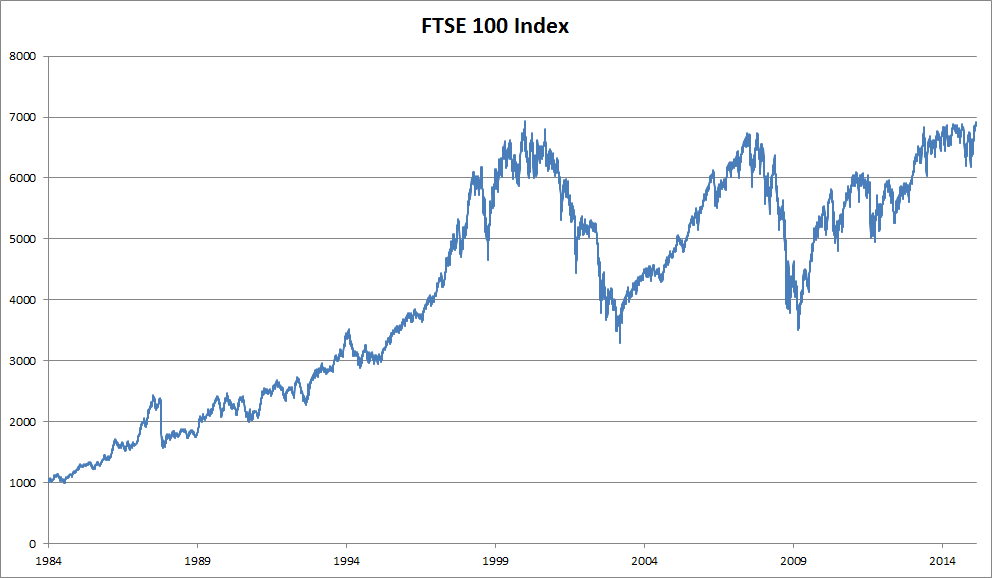
\includegraphics[scale=0.5]{images/app/ftse100.png}
	\caption{FTSE 100 index over 30 years.}
	\label{fig:ftse100}
\end{figure}

Let’s denote the prices by $x_t \geq 0$, i.e. at time $t \in \mathbb{N}$ we observe some price $x_t$. For a trader to do well in the stock market on day $t$ he should want to predict $x_t$ via

$$x_t \sim p(x_t|x_{t-1}, \ldots x_1)$$

\subsubsection{Autoregressive Models}

In order to achieve this, our trader could use a regressor, but there’s just a major problem - the number of inputs, $x_{t-1}, \ldots x_1$ varies, depending on $t$. That is, the number increases with the amount of data that we encounter, and we will need an approximation to make this computationally tractable. Much of what follows in this section will revolve around how to estimate $p(x_t|x_{t-1}, \ldots x_1)$ efficiently. In a nutshell it boils down to two strategies:

\begin{enumerate}
    \item Assume that the potentially rather long sequence $x_{t-1}, \ldots x_1$ is not really necessary. In this case we might content ourselves with some timespan $\tau$ and only use $x_{t-1}, \ldots x_{t-\tau}$ observations. The immediate benefit is that now the number of arguments is always the same, at least for $t > \tau$. This allows us to train a deep network as indicated above. Such models will be called \textit{autoregressive models}, as they quite literally perform regression on themselves.
    \item Another strategy is to try and keep some summary $h_t$ of the past observations around and update that in addition to the actual prediction. This leads to models that estimate $x_t|x_{t-1}, h_{t-1}$ and moreover updates of the form $h_t = g(h_t, x_t)$. Since $h_t$ is never observed, these models are also called \textit{latent autoregressive models}. LSTMs and GRUs are examples of this.
\end{enumerate}

Both cases raise the obvious question of how to generate training data. One typically uses historical observations to predict the next observation given the ones up to right now. Obviously we do not expect time to stand still. However, a common assumption is that while the specific values of $x_t$ might change, at least the dynamics of the time series itself won’t. This is reasonable, since novel dynamics are just that, novel and thus not predictable using data we have so far. Statisticians call dynamics that do not change stationary. Regardless of what we do, we will thus get an estimate of the entire time series via

$$p(x_1, \ldots x_T) = \prod_{t=1}^T p(x_t|x_{t-1}, \ldots x_1)$$

Note that the above considerations still hold if we deal with discrete objects, such as words, rather than numbers. The only difference is that in such a situation we need to use a classifier rather than a regressor to estimate $p(x_t| x_{t-1}, \ldots x_1)$.

\subsubsection{Markov Model}

Recall the approximation that in an autoregressive model we use only $(x_{t-1}, \ldots x_{t-\tau})$ instead of $(x_{t-1}, \ldots x_1)$ to estimate $x_t$. Whenever this approximation is accurate we say that the sequence satisfies a Markov condition. In particular, if $\tau = 1$, we have a first order Markov model and $p(x)$ is given by

$$p(x_1, \ldots x_T) = \prod_{t=1}^T p(x_t|x_{t-1})$$

Such models are particularly nice whenever $x_t$ assumes only discrete values, since in this case dynamic programming can be used to compute values along the chain exactly. For instance, we can compute $x_{t+1}|x_{t-1}$ efficiently using the fact that we only need to take into account a very short history of past observations.

$$p(x_{t+1}|x_{t-1}) = \sum_{x_t} p(x_{t+1}|x_t) p(x_t|x_{t-1})$$

Going into details of dynamic programming is beyond the scope of this section. Control and reinforcement learning algorithms use such tools extensively.

% \subsubsection{Causality}

% In principle, there’s nothing wrong with unfolding $p(x_1, \ldots x_T)$ in reverse order. After all, by conditioning we can always write it via

% $$p(x_1, \ldots x_T) = \prod_{t=T}^1 p(x_t|x_{t+1}, \ldots x_T)$$

% In fact, if we have a Markov model we can obtain a reverse conditional probability distribution, too. In many cases, however, there exists a natural direction for the data, namely going forward in time. It is clear that future events cannot influence the past. Hence, if we change $x_t$, we may be able to influence what happens for $x_{t+1}$ going forward but not the converse. That is, if we change $x_t$, the distribution over past events will not change. Consequently, it ought to be easier to explain $x_{t+1}|x_t$ rather than $x_t|x_{t+1}$. For instance, \citet{Hoyer2008} show that in some cases we can find $x_{t+1} = f(x_t) + \epsilon$ for some additive noise, whereas the converse is not true. This is great news, since it is typically the forward direction that we’re interested in estimating. For more on this topic see for example the book \textit{Elements of Causal Inference}, by \citet{Peters2015}; we are barely scratching the surface of it.

\subsection{Language models}\label{subsec:lang_models}

Text is an important example of sequence data. In fact, we will use natural language models as the basis for many of the examples in this chapter. Given that, it’s worth while discussing some things in a bit more detail. In the following we will view words (or sequences of characters) as a time series of discrete observations. Assuming the words in a text of length $T$ are in turn $w_1, w_2, \ldots, w_T$, then, in the discrete time series, $w_t(1 \leq t \leq T)$ can be considered as the output or label of time step $t$. Given such a sequence, the goal of a language model is to estimate the probability

$$p(w_1, w_2, \ldots, w_T)$$

Language models are incredibly useful. For instance, an ideal language model would be able to generate natural text just on its own, simply by drawing one word at a time $w_t \sim p(w_t|w_{t-1}, \ldots w_1)$. Quite unlike the monkey using a typewriter, all text emerging from such a model would pass as natural language, e.g. English text. Furthermore, it would be sufficient for generating a meaningful dialog, simply by conditioning the text on previous dialog fragments. Clearly we are still very far from designing such a system, since it would need to understand the text rather than just generate grammatically sensible content.

Nonetheless language models are of great service even in their limited form. For instance, the phrases ‘to recognize speech’ and ‘to wreck a nice beach’ sound very similar. This can cause ambiguity in speech recognition, ambiguity that is easily resolved through a language model which rejects the second translation as outlandish. Likewise, in a document summarization algorithm it’s worth while knowing that ‘dog bites man’ is much more frequent than ‘man bites dog’, or that ‘let’s eat grandma’ is a rather disturbing statement, whereas ‘let’s eat, grandma’ is much more benign.

\subsubsection{Estimating a language model}

The obvious question is how we should model a document, or even a sequence of words. We can start by applying basic probability rules:

$$p(w_1, w_2, \ldots, w_T) = \prod_{t=1}^T p(w_t | w_1, \ldots, w_{t-1})$$

For example, the probability of a text sequence containing four tokens consisting of words and punctuation would be given as:

$$p(\mathrm{Statistics}, \mathrm{is},  \mathrm{fun}, \mathrm{.}) =  p(\mathrm{Statistics}) p(\mathrm{is} | \mathrm{Statistics}) p(\mathrm{fun} | \mathrm{Statistics}, \mathrm{is}) p(\mathrm{.} | \mathrm{Statistics}, \mathrm{is}, \mathrm{fun})$$

In order to compute the language model, we need to calculate the probability of words and the conditional probability of a word given the previous few words, i.e. language model parameters. Here, we assume that the training data set is a large text corpus, such as all Wikipedia entries, Project Gutenberg, or all text posted online on the web. The probability of words can be calculated from the relative word frequency of a given word in the training data set.

For example, $p(\mathrm{Statistics})$ can be calculated as the probability of any sentence starting with the word ‘statistics’. A slightly less accurate approach would be to count all occurrences of the word ‘statistics’ and divide it by the total number of words in the corpus. This works fairly well, particularly for frequent words. Moving on, we could attempt to estimate

$$\hat{p}(\mathrm{is}|\mathrm{Statistics}) = \frac{n(\mathrm{Statistics~is})}{n(\mathrm{Statistics})}$$

Here $n(w)$ and $n(w, w')$ are the number of occurrences of singletons and pairs of words respectively. Unfortunately, estimating the probability of a word pair is somewhat more difficult, since the occurrences of ‘Statistics is’ are a lot less frequent. In particular, for some unusual word combinations it may be tricky to find enough occurrences to get accurate estimates. Things take a turn for the worse for 3 word combinations and beyond. There will be many plausible 3-word combinations that we likely will not see in our dataset. Unless we provide some solution to give such word combinations nonzero weight we will not be able to use these as a language model. If the dataset is small or if the words are very rare, we might not find even a single one of them.

A common strategy is to perform some form of Laplace smoothing, that is, adding a small constant to all counts. 
This helps with singletons, e.g. via

$$
\begin{aligned}
    \hat{p}(w) & = \frac{n(w) + \epsilon_1/m}{n + \epsilon_1} \\
    \hat{p}(w'|w) & = \frac{n(w,w') + \epsilon_2 \hat{p}(w')}{n(w) + \epsilon_2} \\
    \hat{p}(w''|w',w) & = \frac{n(w,w',w'') + \epsilon_3 \hat{p}(w',w'')}{n(w,w') + \epsilon_3}
\end{aligned}
$$

Here the coefficients $\epsilon_i > 0$ determine how much we use the estimate for a shorter sequence as a fill-in for longer ones. Moreover, $m$ is the total number of words we encounter. The above is a rather primitive variant of what Kneser-Ney smoothing and Bayesian Non-parametrics can accomplish. 

See e.g. \textit{The Sequence Memoizer} by \citep{Wood2011} for more details of how to accomplish this. Unfortunately models like this get unwieldy rather quickly. First off, we need to store all counts and secondly, this entirely ignores the meaning of the words; for instance, ‘cat’ and ‘feline’ should occur in related contexts. Besides, it is quite difficult to adjust such models to additional context. Lastly, long word sequences are almost certain to be novel, hence a model that simply counts the frequency of previously seen word sequences is bound to perform poorly there.

\subsubsection{Markov Models and n-grams}

Before we discuss solutions involving deep learning we need some more terminology and concepts. Recall our discussion of Markov Models in the previous section. Let’s apply this to language modeling. A distribution over sequences satisfies the Markov property of first order if $p(w_{t+1}|w_t, \ldots w_1) = p(w_{t+1}|w_t)$. Higher orders correspond to longer dependencies. This leads to a number of approximations that we could apply to model a sequence:

$$
\begin{aligned}
p(w_1, w_2, w_3, w_4) &=  p(w_1) p(w_2) p(w_3) p(w_4)\\
p(w_1, w_2, w_3, w_4) &=  p(w_1) p(w_2 | w_1) p(w_3 | w_2) p(w_4 | w_3)\\
p(w_1, w_2, w_3, w_4) &=  p(w_1) p(w_2 | w_1) p(w_3 | w_1, w_2) p(w_4 | w_2, w_3)\\
\end{aligned}
$$

Since they involve one, two or three terms, these are typically referred to as \textit{unigram}, \textit{bigram} and \textit{trigram} models. 
% In the following we will learn how to design better models.

\subsection{Recurrent Neural Networks}\label{subsec:rnn}

In the previous section we introduced $n$-gram models, where the conditional probability of word $w_t$ at position $t$ only depends on the $n-1$ previous words. If we want to check the possible effect of words earlier than $t-(n-1)$ on $w_t$, we need to increase $n$. However, the number of model parameters would also increase exponentially with it, as we need to store $|V|^n$ numbers for a vocabulary $V$. Hence, rather than modeling $p(w_t|w_{t-1}, \ldots w_{t-n+1})$ it is preferable to use a latent variable model in which we have

$$p(w_t|w_{t-1}, \ldots w_1) \approx p(w_t|h_t(w_{t-1}, h_{t-1})).$$

For a sufficiently powerful function $h_t$ this is not an approximation. After
all, $h_t$ could simply store all the data it observed so far. We discussed this
in \cref{subsec:sequence_models}. Let's see why building such models is a bit more tricky than simple autoregressive models where

$$p(w_t|w_{t-1}, \ldots w_1) \approx p(w_t|f(w_{t-1}, \ldots w_{t-n+1}))$$

As a warmup we will review the latter for discrete outputs and $n=2$, i.e. for Markov model of first order. To simplify things further we use a single layer in the design of the RNN. Later on we will see how to add more expressivity efficiently across items.

\subsubsection{Recurrent Networks Without Hidden States}

Let us take a look at a multilayer perceptron with a single hidden layer. Given a mini-batch of instances $\mathbf{X} \in \mathbb{R}^{n \times d}$ with sample size $n$ and $d$ inputs (features or feature vector dimensions). Let the hidden layer's activation function be $\phi$. Hence the hidden layer's output $\mathbf{H} \in \mathbb{R}^{n \times h}$ is calculated as

$$\mathbf{H} = \phi(\mathbf{X} \mathbf{W}_{xh} + \mathbf{b}_h).$$

Here, we have the weight parameter $\mathbf{W}_{xh} \in \mathbb{R}^{d \times h}$, bias parameter $\mathbf{b}_h \in \mathbb{R}^{1 \times h}$, and the number of hidden units $h$, for the hidden layer. 
% Recall that $\mathbf{b}_h$ is just a vector - its values are replicated using the broadcasting mechanism to match those of the matrix-matrix product.

Also note that hidden \textbf{state} and hidden \textbf{layer} refer to two very different concepts. Hidden layers are layers that are hidden from view on the path from input to output. Hidden states are technically speaking inputs to whatever we do at a given step. Instead, they can only be computed by looking at data at previous iterations. In this sense they have much in common with latent variable models in statistics, such as clustering or topic models where e.g. the cluster ID affects the output but cannot be directly observed.

The hidden variable $\mathbf{H}$ is used as the input of the output layer. For classification purposes, such as predicting the next character, the output dimensionality $q$ might e.g. match the number of categories in the classification problem. Lastly the output layer is given by

$$\mathbf{O} = \mathbf{H} \mathbf{W}_{hq} + \mathbf{b}_q.$$

Here, $\mathbf{O} \in \mathbb{R}^{n \times q}$ is the output variable, $\mathbf{W}_{hq} \in \mathbb{R}^{h \times q}$ is the weight parameter, and $\mathbf{b}_q \in \mathbb{R}^{1 \times q}$ is the bias parameter of the output layer.  If it is a classification problem, we can use $\text{softmax}(\mathbf{O})$ to compute the probability distribution of the output category. This is entirely analogous to the regression problem we solved previously in \cref{subsec:sequence_models}, hence we omit details. Suffice it to say that we can pick $(w_t, w_{t-1})$ pairs at random and estimate the parameters $\mathbf{W}$ and $\mathbf{b}$ of our network via autograd and stochastic gradient descent.

\subsubsection{Recurrent Networks with Hidden States}\label{subsubsec:rnn_with_hidden_state}

Matters are entirely different when we have hidden states. Let's look at the structure in some more detail. Assume that $\mathbf{X}_t \in \mathbb{R}^{n \times d}$ is the mini-batch input and $\mathbf{H}_t  \in \mathbb{R}^{n \times h}$ is the hidden variable of time step $t$ from the sequence.  Unlike the multilayer perceptron, here we save the hidden variable $\mathbf{H}_{t-1}$ from the previous time step and introduce a new weight parameter $\mathbf{W}_{hh} \in \mathbb{R}^{h \times h}$, to describe how to use the hidden variable of the previous time step in the current time step. Specifically, the calculation of the hidden variable of the current time step is determined by the input of the current time step together with the hidden variable of the previous time step:

$$\mathbf{H}_t = \phi(\mathbf{X}_t \mathbf{W}_{xh} + \mathbf{H}_{t-1} \mathbf{W}_{hh}  + \mathbf{b}_h)$$

Compared with the multilayer perceptron, we added one more $\mathbf{H}_{t-1} \mathbf{W}_{hh}$ here. From the relationship between hidden variables $\mathbf{H}_t$ and $\mathbf{H}_{t-1}$ of adjacent time steps, we know that those variables captured and retained the sequence's historical information up to the current time step, just like the state or memory of the neural network's current time step. Therefore, such a hidden variable is also called a hidden state. Since the hidden state uses the same definition of the previous time step in the current time step, the computation of the equation above is recurrent, hence the name recurrent neural network (RNN).

There are many different RNN construction methods.  RNNs with a hidden state defined by the equation above are very common. For time step $t$, the output of the output layer is similar to the computation in the multilayer perceptron:

$$\mathbf{O}_t = \mathbf{H}_t \mathbf{W}_{hq} + \mathbf{b}_q$$

RNN parameters include the weight $\mathbf{W}_{xh} \in \mathbb{R}^{d \times h}, \mathbf{W}_{hh} \in \mathbb{R}^{h \times h}$ of the hidden layer with the bias $\mathbf{b}_h \in \mathbb{R}^{1 \times h}$, and the weight $\mathbf{W}_{hq} \in \mathbb{R}^{h \times q}$ of the output layer with the bias $\mathbf{b}_q \in \mathbb{R}^{1 \times q}$. It is worth mentioning that RNNs always use these model parameters, even for different time steps. Therefore, the number of RNN model parameters does not grow as the number of time steps increases.

\cref{fig:rnn} shows the computational logic of an RNN at three adjacent time steps. In time step $t$, the computation of the hidden state can be treated as an entry of a fully connected layer with the activation function $\phi$ after concatenating the input $\mathbf{X}_t$ with the hidden state $\mathbf{H}_{t-1}$ of the previous time step.  The output of the fully connected layer is the hidden state of the current time step $\mathbf{H}_t$. Its model parameter is the concatenation of $\mathbf{W}_{xh}$ and $\mathbf{W}_{hh}$, with a bias of $\mathbf{b}_h$. The hidden state of the current time step $t$ $\mathbf{H}_t$ will participate in computing the hidden state $\mathbf{H}_{t+1}$ of the next time step $t+1$, the result of which will become the input for the fully connected output layer of the current time step.

\begin{figure}[hpt]
	\centering
	\includesvg[scale=0.5]{images/app/rnn.svg}
	\caption{An RNN with a hidden state.}
	\label{fig:rnn}
\end{figure}

As discussed, the computation in the hidden state uses $\mathbf{H}_t = \mathbf{X}_t \mathbf{W}_{xh} + \mathbf{H}_{t-1} \mathbf{W}_{hh}$ to generate an object matching $\mathbf{H}_{t-1}$ in dimensionality. Moreover, we use $\mathbf{H}_t$ to generate the output $\mathbf{O}_t = \mathbf{H}_t \mathbf{W}_{hq}$.

The recurrent network defined above takes observations $X$ and a hidden state $H$ as arguments and uses them to update the hidden state and emit an output $O$. Since this chain could go on for a very long time, training the model with backprop is out of the question (at least without some approximation). After all, this leads to a very long chain of dependencies that would be prohibitive to solve exactly: books typically have more than 100,000 characters and it is unreasonable to assume that the later text relies indiscriminately on all occurrences that happened, say, 10,000 characters in the past. Truncation methods such as BPTT and long short term memory, described later, are useful to address this in a more principled manner. 

\subsubsection{Recurrent networks for language modelling}\label{subsubsec:rnn_lang_modelling}

We conclude this section by illustrating how RNNs can be used to build a language model. For simplicity of illustration we use words rather than characters, since the former are easier to comprehend. Let the number of mini-batch examples be 1, and the sequence of the text be the beginning of our dataset, i.e. “The time Machine by H. G. Wells”. \cref{fig:rnn-train} illustrates how to estimate the next character based on the present and previous characters. During the training process, we run a softmax operation on the output from the output layer for each time step, and then use the cross-entropy loss function to compute the error between the result and the label. Due to the recurrent computation of the hidden state in the hidden layer, the output of time step 3, $\mathbf{O}_3$ is determined by the text sequence “the”, “time”, “machine”. Since the next word of the sequence in the training data is “by”, the loss of time step 3 will depend on the probability distribution of the next word generated based on the sequence “the”, “time”, “machine” and the label “by” of this time step.

\begin{figure}[hpt]
	\centering
	\includesvg[scale=0.8]{images/app/rnn-train.svg}
	\caption{Word-level RNN language model. The input and label sequences are The Time Machine by H. and Time Machine by H. G. respectively.}
	\label{fig:rnn-train}
\end{figure}


The number of words is huge compared to the number of characters. This is why quite often we will use a character-level RNN instead.

% \subsubsection{Sampling}

% During training, we need to read mini-batches of examples and labels at random. Since sequence data is by its very nature sequential, we need to address the issue of processing it. Consider the beginning of the book we just processed. If we want to split it up into sequences of 5 symbols each, we have quite some freedom since we could pick an arbitrary offset.

% \begin{figure}[hpt]
% 	\centering
% 	\includesvg{images/app/timemachine-5gram.svg}
% 	\caption{ifferent offsets lead to different subsequences when splitting up text.}
% 	\label{fig:timemachine-5gram}
% \end{figure}

% In fact, any one of these offsets is fine. Hence, which one should we pick? In fact, all of them are equally good. But if we pick all offsets we end up with rather redundant data due to overlap, particularly if the sequences are long. Picking just a random set of initial positions is no good either since it does not guarantee uniform coverage of the array. For instance, if we pick $n$ elements at random out of a set of $n$ with random replacement, the probability for a particular element not being picked is $(1-1/n)^n \to e^{-1}$. This means that we cannot expect uniform coverage this way. Even randomly permuting a set of all offsets does not offer good guarantees. Instead we can use a simple trick to get both coverage and randomness: use a random offset, after which one uses the terms sequentially. This can be done both for random sampling and sequential partitioning.

% \paragraph{Random sampling}

% Randomly generates a minibatch from the data each time. In random sampling, each example is a sequence arbitrarily captured on the original sequence. The positions of two adjacent random mini-batches on the original sequence are not necessarily adjacent. The target is to predict the next character based on what we’ve seen so far, hence the labels are the original sequence, shifted by one character. Note that this is not recommended for latent variable models, since we do not have access to the hidden state prior to seeing the sequence. 

% \paragraph{Sequential partitioning}

% In addition to random sampling of the original sequence, we can also make the positions of two adjacent random mini-batches adjacent in the original sequence. Now, we can use a hidden state of the last time step of a mini-batch to initialize the hidden state of the next mini-batch, so that the output of the next mini-batch is also dependent on the input of the mini-batch, with this pattern continuing in subsequent mini-batches. This has two effects on the implementation of a recurrent neural network. On the one hand, when training the model, we only need to initialize the hidden state at the beginning of each epoch. On the other hand, when multiple adjacent mini-batches are concatenated by passing hidden states, the gradient calculation of the model parameters will depend on all the mini-batch sequences that are concatenated. In the same epoch as the number of iterations increases, the costs of gradient calculation rise. So that the model parameter gradient calculations only depend on the mini-batch sequence read by one iteration, we can separate the hidden state from the computational graph before reading the mini-batch (this can be done by detaching the graph).

% \subsection{Training Recurrent Networks: Backpropagation Through Time (BPTT)}

% In this section we will delve a bit more deeply into the details of backpropagation for sequence models and why (and how) the math works.

% Forward propagation in a recurrent neural network is relatively straightforward. Back-propagation through time (BPTT) is actually a specific application of back propagation in recurrent neural networks. It requires us to expand the recurrent neural network one time step at a time to obtain the dependencies between model variables and parameters. Then, based on the chain rule, we apply back propagation to compute and store gradients. Since sequences can be rather long this means that the dependency can be rather lengthy. E.g. for a sequence of 1000 characters the first symbol could potentially have significant influence on the symbol at position 1000. This is not really computationally feasible (it takes too long and requires too much memory) and it requires over 1000 matrix-vector products before we would arrive at that very elusive gradient. This is a process fraught with computational and statistical uncertainty. In the following we will address what happens and how to address this in practice.

% \subsubsection{A Simplified Recurrent Network}

% We start with a simplified model of how an RNN works. This model ignores details about the specifics of the hidden state and how it is being updated. These details are immaterial to the analysis and would only serve to clutter the notation and make it look more intimidating.

% $$h_t = f(x_t, h_{t-1}, w) \text{ and } o_t = g(h_t, w)$$

% Here $h_t$ denotes the hidden state, $x_t$ the input and $o_t$ the output. We have a chain of values $\{\ldots (h_{t-1}, x_{t-1}, o_{t-1}), (h_{t}, x_{t}, o_t), \ldots\}$ that depend on each other via recursive computation. The forward pass is fairly straightforward. All we need is to loop through the $(x_t, h_t, o_t)$ triples one step at a time. This is then evaluated by an objective function measuring the discrepancy between outputs $o_t$ and some desired target $y_t$

% $$L(x,y, w) = \sum_{t=1}^T l(y_t, o_t)$$

% For backpropagation matters are a bit more tricky. Let’s compute the gradients with regard to the parameters $w$ of the objective function $L$. We get that

% $$
% \begin{aligned}
% \partial_{w} L & = \sum_{t=1}^T \partial_w l(y_t, o_t) \\
%     & = \sum_{t=1}^T \partial_{o_t} l(y_t, o_t) \left[\partial_w g(h_t, w) + \partial_{h_t} g(h_t,w) \partial_w h_t\right]
% \end{aligned}
% $$

% The first part of the derivative is easy to compute (this is after all the instantaneous loss gradient at time $t$). The second part is where things get tricky, since we need to compute the effect of the parameters on $h_t$. For each term we have the recursion:

% $$
% \begin{aligned}
%     \partial_w h_t & = \partial_w f(x_t, h_{t-1}, w) + \partial_h f(x_t, h_{t-1}, w) \partial_w h_{t-1} \\
%     & = \sum_{i=t}^1 \left[\prod_{j=t}^i \partial_h f(x_j, h_{j-1}, w) \right] \partial_w f(x_{i}, h_{i-1}, w)
% \end{aligned}
% $$

% This chain can get very long whenever $t$ is large. While we can use the chain rule to compute $\partial_w h_t$ recursively, this might not be ideal. Let’s discuss a number of strategies for dealing with this problem:

% \textbf{Compute the full sum}. This is very slow and gradients can blow up, since subtle changes in the initial conditions can potentially affect the outcome a lot. That is, we could see things similar to the butterfly effect where minimal changes in the initial conditions lead to disproportionate changes in the outcome. This is actually quite undesirable in terms of the model that we want to estimate. After all, we are looking for robust estimators that generalize well. Hence this strategy is almost never used in practice.

% \textbf{Truncate the sum after $\tau$ steps}. This is what we have been discussing so far. This leads to an approximation of the true gradient, simply by terminating the sum above at $\partial_w h_{t-\tau}$. The approximation error is thus given by $\partial_h f(x_t, h_{t-1}, w) \partial_w h_{t-1}$ (multiplied by a product of gradients involving $\partial_h f$). In practice this works quite well. It is what is commonly referred to as truncated BPTT (backpropgation through time). One of the consequences of this is that the model focuses primarily on short-term influence rather than long-term consequences. This is actually desirable, since it biases the estimate towards simpler and more stable models.

% % \subsubsection{The Computational Graph}

% % In order to visualize the dependencies between model variables and parameters during computation in a recurrent neural network, we can draw a computational graph for the model, as shown below. For example, the computation of the hidden states of time step 3 $\mathbf{h}_3$ depends on the model parameters $\mathbf{W}_{hx}$ and $\mathbf{W}_{hh}$, the hidden state of the last time step $\mathbf{h}_2$, and the input of the current time step $\mathbf{x}_3.$

% % \begin{figure}[hpt]
% % 	\centering
% % 	\includesvg[scale=0.8]{images/app/rnn-bptt.svg}
% % 	\caption{Computational dependencies for a recurrent neural network model with three time steps. Boxes represent variables (not shaded) or parameters (shaded) and circles represent operators.}
% % 	\label{fig:rnn-bptt}
% % \end{figure}

% % \subsubsection{BPTT in Detail}

% % Now that we discussed the general principle let’s discuss BPTT in detail, distinguishing between different sets of weight matrices $(\mathbf{W}_{hx}, \mathbf{W}_{hh} and \mathbf{W}_{oh})$ in a simple linear latent variable model:

% % $$\mathbf{h}_t = \mathbf{W}_{hx} \mathbf{x}_t + \mathbf{W}_{hh} \mathbf{h}_{t-1} \text{ and }\mathbf{o}_t = \mathbf{W}_{oh} \mathbf{h}_t$$

% % We compute gradients $\partial L/\partial \mathbf{W}_{hx}$, $\partial L/\partial \mathbf{W}_{hh}$, and $\partial L/\partial \mathbf{W}_{oh}$ for $L(\mathbf{x}, \mathbf{y}, \mathbf{W}) = \sum_{t=1}^T l(\mathbf{o}_t, y_t)$. Taking the derivatives with respect to $W_{oh}$ is fairly straightforward and we obtain

% % $$\partial_{\mathbf{W}_{oh}} L = \sum_{t=1}^T \mathrm{prod}
% % \left(\partial_{\mathbf{o}_t} l(\mathbf{o}_t, y_t), \mathbf{h}_t\right)$$

% % The dependency on $\mathbf{W}_{hx}$ and $\mathbf{W}_{hh}$ is a bit more tricky since it involves a chain of derivatives. We begin with

% % $$
% % \begin{aligned}
% % \partial_{\mathbf{W}_{hh}} L & = \sum_{t=1}^T \mathrm{prod}
% % \left(\partial_{\mathbf{o}_t} l(\mathbf{o}_t, y_t), \mathbf{W}_{oh}, \partial_{\mathbf{W}_{hh}} \mathbf{h}_t\right) \\
% % \partial_{\mathbf{W}_{hx}} L & = \sum_{t=1}^T \mathrm{prod}
% % \left(\partial_{\mathbf{o}_t} l(\mathbf{o}_t, y_t), \mathbf{W}_{oh}, \partial_{\mathbf{W}_{hx}} \mathbf{h}_t\right)
% % \end{aligned}
% % $$

% % After all, hidden states depend on each other and on past inputs. The key quantity is how past hidden states affect future hidden states.

% % $$\partial_{\mathbf{h}_t} \mathbf{h}_{t+1} = \mathbf{W}_{hh}^\top \text{ and thus } \partial_{\mathbf{h}_t} \mathbf{h}_T = \left(\mathbf{W}_{hh}^\top\right)^{T-t}$$

% % Chaining terms together yields

% % $$
% % \begin{aligned}
% % \partial_{\mathbf{W}_{hh}} \mathbf{h}_t & = \sum_{j=1}^t \left(\mathbf{W}_{hh}^\top\right)^{t-j} \mathbf{h}_j \\
% % \partial_{\mathbf{W}_{hx}} \mathbf{h}_t & = \sum_{j=1}^t \left(\mathbf{W}_{hh}^\top\right)^{t-j} \mathbf{x}_j.
% % \end{aligned}
% % $$

% % A number of things follow from this potentially very intimidating expression. Firstly, it pays to store intermediate results, i.e. powers of $\mathbf{W}_{hh}$ as we work our way through the terms of the loss function $L$. Secondly, this simple linear example already exhibits some key problems of long sequence models: it involves potentially very large powers $\mathbf{W}_{hh}^j$. In it, eigenvalues smaller than 1 vanish for large $j$ and eigenvalues larger than 1 diverge. This is numerically unstable and gives undue importance to potentially irrelevant past detail. One way to address this is to truncate the sum at a computationally convenient size. Later on in this chapter we will see how more sophisticated sequence models such as LSTMs can alleviate this further. In code, this truncation is effected by detaching the gradient after a given number of steps.

\subsection{Gated Recurrent Units (GRU)}\label{subsec:gru}

In the previous section we discussed how gradients are calculated in a recurrent neural network. In particular we found that long products of matrices can lead to vanishing or divergent gradients. Let’s briefly think about what such gradient anomalies mean in practice:

We might encounter a situation where an early observation is highly significant for predicting all future observations. Consider the somewhat contrived case where the first observation contains a checksum and the goal is to discern whether the checksum is correct at the end of the sequence. In this case the influence of the first token is vital. We would like to have some mechanism for storing vital early information in a memory cell. Without such a mechanism we will have to assign a very large gradient to this observation, since it affects all subsequent observations.
We might encounter situations where some symbols carry no pertinent observation. For instance, when parsing a webpage there might be auxiliary HTML code that is irrelevant for the purpose of assessing the sentiment conveyed on the page. We would like to have some mechanism for skipping such symbols in the latent state representation.
We might encounter situations where there is a logical break between parts of a sequence. For instance there might be a transition between chapters in a book, a transition between a bear and a bull market for securities, etc.; In this case it would be nice to have a means of resetting our internal state representation.
A number of methods have been proposed to address this. One of the earliest is the Long Short Term Memory (LSTM) of \citep{Hochreiter1997}, which we will discuss in \cref{subsec:lstm}. The Gated Recurrent Unit (GRU) of \citet{Cho2014}, is a slightly more streamlined variant that often offers comparable performance and is significantly faster to compute. See also \citep{Chung2014} for more details. Due to its simplicity we start with the GRU.

\subsubsection{Gating the Hidden State}

The key distinction between regular RNNs and GRUs is that the latter support gating of the hidden state. This means that we have dedicated mechanisms for when the hidden state should be updated and also when it should be reset. These mechanisms are learned and they address the concerns listed above. For instance, if the first symbol is of great importance we will learn not to update the hidden state after the first observation. Likewise, we will learn to skip irrelevant temporary observations. Lastly, we will learn to reset the latent state whenever needed. We discuss this in detail below.

\paragraph{Reset Gates and Update Gates}

The first thing we need to introduce are reset and update gates. We engineer them to be vectors with entries in $(0,1)$ such that we can perform convex combinations, e.g.\ of a hidden state and an alternative. For instance, a reset variable would allow us to control how much of the previous state we might still want to remember. Likewise, an update variable would allow us to control how much of the new state is just a copy of the old state.

We begin by engineering gates to generate these variables. \cref{fig:gru_1} illustrates the inputs for both reset and update gates in a GRU, given the current time step input $\mathbf{X}_t$ and the hidden state of the previous time step $\mathbf{H}_{t-1}$. The output is given by a fully connected layer with a sigmoid as its activation function.

\begin{figure}[hpt]
	\centering
	\includesvg[scale=0.8]{images/app/gru_1.svg}
	\caption{Reset and update gate in a GRU.}
	\label{fig:gru_1}
\end{figure}

Here, we assume there are $h$ hidden units and, for a given time step $t$, the mini-batch input is $\mathbf{X}_t \in \mathbb{R}^{n \times d}$ (number of examples: $n$, number of inputs: $d$) and the hidden state of the last time step is $\mathbf{H}_{t-1} \in \mathbb{R}^{n \times h}$. Then, the reset gate $\mathbf{R}_t \in \mathbb{R}^{n \times h}$ and update gate $\mathbf{Z}_t \in \mathbb{R}^{n \times h}$ are computed as follows:

$$
\begin{aligned}
\mathbf{R}_t = \sigma(\mathbf{X}_t \mathbf{W}_{xr} + \mathbf{H}_{t-1} \mathbf{W}_{hr} + \mathbf{b}_r)\\
\mathbf{Z}_t = \sigma(\mathbf{X}_t \mathbf{W}_{xz} + \mathbf{H}_{t-1} \mathbf{W}_{hz} + \mathbf{b}_z)
\end{aligned}
$$

Here, $\mathbf{W}_{xr}, \mathbf{W}_{xz} \in \mathbb{R}^{d \times h}$ and $\mathbf{W}_{hr}, \mathbf{W}_{hz} \in \mathbb{R}^{h \times h}$ are weight parameters and $\mathbf{b}_r, \mathbf{b}_z \in \mathbb{R}^{1 \times h}$ are biases. We use a sigmoid function to transform values to the interval $(0,1)$.

\paragraph{Reset Gate in Action}

We begin by integrating the reset gate with a regular latent state updating mechanism. In a conventional deep RNN we would have an update of the form

$$\mathbf{H}_t = \tanh(\mathbf{X}_t \mathbf{W}_{xh} + \mathbf{H}_{t-1}\mathbf{W}_{hh} + \mathbf{b}_h)$$

This is essentially identical to the discussion of the previous section, albeit with a nonlinearity in the form of $\tanh$ to ensure that the values of the hidden state remain in the interval $(-1, 1)$.
If we want to be able to reduce the influence of previous states we can multiply $\mathbf{H}_{t-1}$ with $\mathbf{R}_t$ elementwise. Whenever the entries in $\mathbf{R}_t$ are close to $1$ we recover a conventional deep RNN. For all entries of $\mathbf{R}_t$ that are close to $0$ the hidden state is the result of an MLP with $\mathbf{X}_t$ as input. Any pre-existing hidden state is thus 'reset' to defaults. This leads to the following candidate for a new hidden state (it is a \textit{candidate} since we still need to incorporate the action of the update gate).

$$\tilde{\mathbf{H}}_t = \tanh(\mathbf{X}_t \mathbf{W}_{xh} + \left(\mathbf{R}_t \odot \mathbf{H}_{t-1}\right) \mathbf{W}_{hh} + \mathbf{b}_h)$$

\cref{fig:gru_2} illustrates the computational flow after applying the reset gate. The symbol $\odot$ indicates pointwise multiplication between tensors.

\begin{figure}[hpt]
	\centering
	\includesvg[scale=0.8]{images/app/gru_2.svg}
	\caption{Candidate hidden state computation in a GRU. The multiplication is carried out elementwise.}
	\label{fig:gru_2}
\end{figure}

\paragraph{Update Gate in Action}

Next we need to incorporate the effect of the update gate. This determines the extent to which the new state $\mathbf{H}_t$ is just the old state $\mathbf{H}_{t-1}$ and by how much the new candidate state $\tilde{\mathbf{H}}_t$ is used. The gating variable $\mathbf{Z}_t$ can be used for this purpose, simply by taking elementwise convex combinations between both candidates. This leads to the final update equation for the GRU.

$$\mathbf{H}_t = \mathbf{Z}_t \odot \mathbf{H}_{t-1}  + (1 - \mathbf{Z}_t) \odot \tilde{\mathbf{H}}_t$$

\begin{figure}[hpt]
	\centering
	\includesvg[scale=0.8]{images/app/gru_3.svg}
	\caption{Hidden state computation in a GRU. As before, the multiplication is carried out elementwise.}
	\label{fig:gru_3}
\end{figure}

Whenever the update gate is close to $1$ we simply retain the old state. In this case the information from $\mathbf{X}_t$ is essentially ignored, effectively skipping time step $t$ in the dependency chain. Whenever it is close to $1$ the new latent state $\mathbf{H}_t$ approaches the candidate latent state $\tilde{\mathbf{H}}_t$. These designs can help cope with the vanishing gradient problem in RNNs and better capture dependencies for time series with large time step distances. In summary GRUs have the following two distinguishing features:

\begin{itemize}
    \item Reset gates help capture short-term dependencies in time series.
    \item Update gates help capture long-term dependencies in time series.
\end{itemize}

\subsection{Long Short Term Memory (LSTM)}\label{subsec:lstm}

The challenge to address long-term information preservation and short-term input skipping in latent variable models has existed for a long time. One of the earliest approaches to address this was the LSTM by Hochreiter and Schmidhuber, 1997. It shares many of the properties of the Gated Recurrent Unit (GRU) and predates it by almost two decades. Its design is slightly more complex.

Arguably it is inspired by logic gates of a computer. To control a memory cell we need a number of gates. One gate is needed to read out the entries from the cell (as opposed to reading any other cell). We will refer to this as the \textit{output} gate. A second gate is needed to decide when to read data into the cell. We refer to this as the \textit{input} gate. Lastly, we need a mechanism to reset the contents of the cell, governed by a \textit{forget} gate. The motivation for such a design is the same as before, namely to be able to decide when to remember and when to ignore inputs into the latent state via a dedicated mechanism. Let’s see how this works in practice.

\subsubsection{Gated Memory Cells}

Three gates are introduced in LSTMs: the input gate, the forget gate, and the output gate. In addition to that we introduce memory cells that take the same shape as the hidden state. Strictly speaking this is just a fancy version of a hidden state, custom engineered to record additional information.

\paragraph{Input Gates, Forget Gates and Output Gates}

Just like with GRUs, the data feeding into the LSTM gates is the input at the current time step $\mathbf{X}_t$ and the hidden state of the previous time step $\mathbf{H}_{t-1}$. These inputs are processed by a fully connected layer and a sigmoid activation function to compute the values of input, forget and output gates. As a result, the three gate elements all have a value range of $[0,1]$.

\begin{figure}[hpt]
	\centering
	\includesvg[scale=0.8]{images/app/lstm_0.svg}
	\caption{Calculation of input, forget, and output gates in an LSTM.}
	\label{fig:lstm_0}
\end{figure}

We assume there are $h$ hidden units and that the minibatch is of size $n$. Thus
the input is $\mathbf{X}_t \in \mathbb{R}^{n \times d}$ (number of examples:
$n$, number of inputs: $d$) and the hidden state of the last time step is $\mathbf{H}_{t-1} \in \mathbb{R}^{n \times h}$. Correspondingly the gates are defined as follows: the input gate is $\mathbf{I}_t \in \mathbb{R}^{n \times h}$, the forget gate is $\mathbf{F}_t \in \mathbb{R}^{n \times h}$, and the output gate is $\mathbf{O}_t \in \mathbb{R}^{n \times h}$. They are calculated as follows:

$$
\begin{aligned}
\mathbf{I}_t &= \sigma(\mathbf{X}_t \mathbf{W}_{xi} + \mathbf{H}_{t-1} \mathbf{W}_{hi} + \mathbf{b}_i),\\
\mathbf{F}_t &= \sigma(\mathbf{X}_t \mathbf{W}_{xf} + \mathbf{H}_{t-1} \mathbf{W}_{hf} + \mathbf{b}_f),\\
\mathbf{O}_t &= \sigma(\mathbf{X}_t \mathbf{W}_{xo} + \mathbf{H}_{t-1} \mathbf{W}_{ho} + \mathbf{b}_o),
\end{aligned}
$$

$\mathbf{W}_{xi}, \mathbf{W}_{xf}, \mathbf{W}_{xo} \in \mathbb{R}^{d \times h}$ and $\mathbf{W}_{hi}, \mathbf{W}_{hf}, \mathbf{W}_{ho} \in \mathbb{R}^{h \times h}$ are weight parameters and $\mathbf{b}_i, \mathbf{b}_f, \mathbf{b}_o \in \mathbb{R}^{1 \times h}$ are bias parameters.

\paragraph{Candidate Memory Cell}

Next we design a memory cell. Since we haven't specified the action of the various gates yet, we first introduce a \textit{candidate} memory cell $\tilde{\mathbf{C}}_t \in \mathbb{R}^{n \times h}$. Its computation is similar to the three gates described above, but using a $\tanh$ function with a value range for $[-1, 1]$ as activation function. This leads to the following equation at time step $t$.

$$\tilde{\mathbf{C}}_t = \text{tanh}(\mathbf{X}_t \mathbf{W}_{xc} + \mathbf{H}_{t-1} \mathbf{W}_{hc} + \mathbf{b}_c)$$

Here $\mathbf{W}_{xc} \in \mathbb{R}^{d \times h}$ and $\mathbf{W}_{hc} \in \mathbb{R}^{h \times h}$ are weights and $\mathbf{b}_c \in \mathbb{R}^{1 \times h}$ is a bias.

\begin{figure}[hpt]
	\centering
	\includesvg[scale=0.8]{images/app/lstm_1.svg}
	\caption{Computation of candidate memory cells in LSTM.}
	\label{fig:lstm_1}
\end{figure}


\paragraph{Memory Cell}

In GRUs we had a single mechanism to govern input and forgetting. Here we have two parameters, $\mathbf{I}_t$ which governs how much we take new data into account via $\tilde{\mathbf{C}}_t$ and the forget parameter $\mathbf{F}_t$ which addresses how much we of the old memory cell content $\mathbf{C}_{t-1} \in \mathbb{R}^{n \times h}$ we retain. Using the same pointwise multiplication trick as before we arrive at the following update equation.

$$\mathbf{C}_t = \mathbf{F}_t \odot \mathbf{C}_{t-1} + \mathbf{I}_t \odot \tilde{\mathbf{C}}_t.$$

If the forget gate is always approximately 1 and the input gate is always approximately 0, the past memory cells will be saved over time and passed to the current time step. This design was introduced to alleviate the vanishing gradient problem and to better capture dependencies for time series with long range dependencies. We thus arrive at the following flow diagram.

\begin{figure}[hpt]
	\centering
	\includesvg[scale=0.8]{images/app/lstm_2.svg}
	\caption{Computation of memory cells in an LSTM. Here, the multiplication is carried out element-wise.}
	\label{fig:lstm_2}
\end{figure}

\paragraph{Hidden States}

Lastly we need to define how to compute the hidden state $\mathbf{H}_t \in \mathbb{R}^{n \times h}$. This is where the output gate comes into play. In the LSTM it is simply a gated version of the $\tanh$ of the memory cell. This ensures that the values of $\mathbf{H}_t$ are always in the interval $[-1, 1]$. Whenever the output gate is $1$ we effectively pass all memory information through to the predictor whereas for output $0$ we retain all information only within the memory cell and perform no further processing. \cref{fig:lstm_3} has a graphical illustration of the data flow.

$$\mathbf{H}_t = \mathbf{O}_t \odot \tanh(\mathbf{C}_t).$$

\begin{figure}[hpt]
	\centering
	\includesvg[scale=0.8]{images/app/lstm_3.svg}
	\caption{Computation of the hidden state. Multiplication is element-wise.}
	\label{fig:lstm_3}
\end{figure}

\subsection{Deep Recurrent Neural Networks}

Up to now, we only discussed recurrent neural networks with a single unidirectional hidden layer. In it the specific functional form of how latent variables and observations interact was rather arbitrary. This isn't a big problem as long as we have enough flexibility to model different types of interactions. With a single layer, however, this can be quite challenging. In the case of the perceptron we fixed this problem by adding more layers. Within RNNs this is a bit more tricky, since we first need to decide how and where to add extra nonlinearity. Our discussion below focuses primarily on LSTMs but it applies to other sequence models, too.

\begin{itemize}
    \item We could add extra nonlinearity to the gating mechansims. That is, instead of using a single perceptron we could use multiple layers. This leaves the \textit{mechanism} of the LSTM unchanged. Instead it makes it more sophisticated. This would make sense if we were led to believe that the LSTM mechanism describes some form of universal truth of how latent variable autoregressive models work.
    \item We could stack multiple layers of LSTMs on top of each other. This results in a mechanism that is more flexible, due to the combination of several simple layers. In particular, data might be relevant at different levels of the stack. For instance, we might want to keep high-level data about financial market conditions (bear or bull market) available at a high level, whereas at a lower level we only record shorter-term temporal dynamics.
\end{itemize}

Beyond all this abstract discussion it is probably easiest to understand the family of models we are interested in by reviewing the diagram below. It describes a deep recurrent neural network with $L$ hidden layers. Each hidden state is continuously passed to the next time step of the current layer and the next layer of the current time step.

\begin{figure}[hpt]
	\centering
	\includesvg[scale=0.8]{images/app/deep-rnn.svg}
	\caption{Architecture of a deep recurrent neural network.}
	\label{fig:deep-rnn}
\end{figure}

\subsubsection{Functional Dependencies}

At time step $t$ we assume that we have a minibatch $\mathbf{X}_t \in \mathbb{R}^{n \times d}$ (number of examples: $n$, number of inputs: $d$). The hidden state of hidden layer $\ell$ ($\ell=1,\ldots,T$) is $\mathbf{H}_t^{(\ell)}  \in \mathbb{R}^{n \times h}$ (number of hidden units: $h$), the output layer variable is $\mathbf{O}_t \in \mathbb{R}^{n \times q}$ (number of outputs: $q$) and a hidden layer activation function $f_l$ for layer $l$. We compute the hidden state of layer $1$ as before, using $\mathbf{X}_t$ as input. For all subsequent layers the hidden state of the previous layer is used in its place.

$$\begin{aligned}
\mathbf{H}_t^{(1)} & = f_1\left(\mathbf{X}_t, \mathbf{H}_{t-1}^{(1)}\right) \\
\mathbf{H}_t^{(l)} & = f_l\left(\mathbf{H}_t^{(l-1)}, \mathbf{H}_{t-1}^{(l)}\right)
\end{aligned}$$

Finally, the output of the output layer is only based on the hidden state of hidden layer $L$. We use the output function $g$ to address this:

$$\mathbf{O}_t = g \left(\mathbf{H}_t^{(L)}\right)$$

Just as with multilayer perceptrons, the number of hidden layers $L$ and number of hidden units $h$ are hyper parameters. In particular, we can pick a regular RNN, a GRU or an LSTM to implement the model.

% \subsection{Bidirectional Recurrent Neural Networks}

% So far we assumed that our goal is to model the next word given what we've seen so far, e.g. in the context of a time series or in the context of a language model. While this is a typical scenario, it is not the only one we might encounter. To illustrate the issue, consider the following three tasks of filling in the blanks in a text:

% \begin{verbatim}
% I am _____
% I am _____ very hungry.
% I am _____ very hungry, I could eat half a pig.    
% \end{verbatim}

% Depending on the amount of information available we might fill the blanks with very different words such as 'happy', 'not', and 'very'. Clearly the end of the phrase (if available) conveys significant information about which word to pick. A sequence model that is incapable of taking advantage of this will perform poorly on related tasks. For instance, to do well in named entity recognition (e.g. to recognize whether 'Green' refers to 'Mr. Green' or to the color) longer-range context is equally vital. To get some inspiration for addressing the problem let's take a detour to graphical models.

% \subsubsection{Dynamic Programming}

% This section serves to illustrate the problem. The specific technical details do not matter for understanding the deep learning counterpart but they help in motivating why one might use deep learning and why one might pick specific architectures.

% If we want to solve the problem using graphical models we could for instance design a latent variable model as follows: we assume that there exists some latent variable $h_t$ which governs the emissions $x_t$ that we observe via $p(x_t|h_t)$. Moreover, the transitions $h_t \to h_{t+1}$ are given by some state transition probability $p(h_t|h_{t-1})$. The graphical model then looks as follows:

% \begin{figure}[hpt]
% 	\centering
% 	\includesvg[scale=0.8]{images/app/hmm.svg}
% 	\caption{Hidden Markov Model.}
% 	\label{fig:hmm}
% \end{figure}

% For a sequence of $T$ observations we have thus the following joint probability distribution over observed and hidden states:

% $$p(x,h) = p(h_1) p(x_1|h_1) \prod_{i=2}^T p(h_t|h_{t-1}) p(x_t|h_t)$$

% Now assume that we observe all $x_i$ with the exception of some $x_j$ and it is our goal to compute $p(x_j|x^{-j})$. To accomplish this we need to sum over all possible choices of $h = (h_1, \ldots, h_T)$. In case $h_i$ can take on $k$ distinct values this means that we need to sum over $k^T$ terms - mission impossible! Fortunately there's an elegant solution for this: \textbf{dynamic programming}. To see how it works consider summing over the first two hidden variable $h_1$ and $h_2$. This yields:

% $$\begin{aligned}
%     p(x) & = \sum_h p(h_1) p(x_1|h_1) \prod_{i=2}^T p(h_t|h_{t-1}) p(x_t|h_t) \\
%     & = \sum_{h_2, \ldots h_T} \underbrace{\left[\sum_{h_1} p(h_1) p(x_1|h_1) p(h_2|h_1)\right]}_{=: \pi_2(h_2)}
%     p(x_2|h_2) \prod_{i=2}^T p(h_t|h_{t-1}) p(x_t|h_t) \\
%     & = \sum_{h_3, \ldots h_T} \underbrace{\left[\sum_{h_2} \pi_2(h_2) p(x_2|h_2) p(h_3|h_2)\right]}_{=: \pi_3(h_3)}
%     p(x_3|h_3) \prod_{i=3}^T p(h_t|h_{t-1}) p(x_t|h_t)
% \end{aligned}$$

% In general we have the \textit{forward} recursion

% $$\pi_{t+1}(h_{t+1}) = \sum_{h_t} \pi_t(h_t) p(x_t|h_t) p(h_{t+1}|h_1)$$

% The recursion is initialized as $\pi_1(h_1) = p(h_1)$. In abstract terms this can be written as $\pi_{t+1} = f(\pi_t, x_t)$, where $f$ is some learned function. This looks very much like the update equation in the hidden variable models we discussed so far in the context of RNNs. Entirely analogously to the forward recursion we can also start a backwards recursion. This yields:

% $$\begin{aligned}
%     p(x) & = \sum_h \prod_{i=1}^{T-1} p(h_t|h_{t-1}) p(x_t|h_t) \cdot p(h_T|h_{T-1}) p(x_T|h_T) \\
%     & = \sum_{h_1, \ldots h_{T-1}} \prod_{i=1}^{T-1} p(h_t|h_{t-1}) p(x_t|h_t) \cdot
%     \underbrace{\left[\sum_{h_T} p(h_T|h_{T-1}) p(x_T|h_T)\right]}_{=: \rho_{T-1}(h_{T-1})} \\
%     & = \sum_{h_1, \ldots h_{T-2}} \prod_{i=1}^{T-2} p(h_t|h_{t-1}) p(x_t|h_t) \cdot
%     \underbrace{\left[\sum_{h_{T-1}} p(h_{T-1}|h_{T-2}) p(x_{T-1}|h_{T-1})\right]}_{=: \rho_{T-2}(h_{T-2})}
% \end{aligned}$$

% We can thus write the \textit{backward} recursion as

% $$\rho_{t-1}(h_{t-1})= \sum_{h_{t}} p(h_{t}|h_{t-1}) p(x_{t}|h_{t})$$

% with initialization $\rho_T(h_T) = 1$. These two recursions allow us to sum over $T$ variables in $O(kT)$ (linear) time over all values of $(h_1, \ldots h_T)$ rather than in exponential time. This is one of the great benefits of probabilistic inference with graphical models. It is a very special instance of the [Generalized Distributive Law](https://authors.library.caltech.edu/1541/1/AJIieeetit00.pdf) proposed in 2000 by Aji and McEliece. Combining both forward and backward pass we are able to compute

% $$p(x_j|x_{-j}) \propto \sum_{h_j} \pi_j(h_j) \rho_j(h_j) p(x_j|h_j).$$

% Note that in abstract terms the backward recursion can be written as $\rho_{t-1} = g(\rho_t, x_t)$, where $g$ is some learned function. Again, this looks very much like an update equation, just running backwards unlike what we've seen so far in RNNs. And, indeed, HMMs benefit from knowing future data when it is available. Signal processing scientists distinguish between the two cases of knowing and not knowing future observations as filtering vs. smoothing.

% \subsubsection{Bidirectional Model}

% If we want to have a mechanism in RNNs that offers comparable look-ahead ability as in HMMs we need to modify the recurrent net design we’ve seen so far. Fortunately this is easy (conceptually). Instead of running an RNN only in forward mode starting from the first symbol we start another one from the last symbol running back to front. Bidirectional recurrent neural networks add a hidden layer that passes information in a backward direction to more flexibly process such information. The figure below illustrates the architecture of a bidirectional recurrent neural network with a single hidden layer.

% \begin{figure}[hpt]
% 	\centering
% 	\includesvg{images/app/birnn.svg}
% 	\caption{Architecture of a bidirectional recurrent neural network.}
% 	\label{fig:birnn}
% \end{figure}

% In fact, this is not too dissimilar to the forward and backward recurrences we encountered above. The main distinction is that in the previous case these equations had a specific statistical meaning. Now they’re devoid of such easily accessible interpretation and we can just treat them as generic functions. This transition epitomizes many of the principles guiding the design of modern deep networks - use the type of functional dependencies common to classical statistical models and use them in a generic form.

% \paragraph{Definition}

% Bidirectional RNNs were introduced by \citet{Schuster1997}. For a detailed discussion of the various architectures see also the paper by \citet{Graves2005}. Let's look at the specifics of such a network. For a given time step $t$, the mini-batch input is $\mathbf{X}_t \in \mathbb{R}^{n \times d}$ (number of examples: $n$, number of inputs: $d$) and the hidden layer activation function is $\phi$. In the bidirectional architecture:
% We assume that the forward and backward hidden states for this time step are $\overrightarrow{\mathbf{H}}_t  \in \mathbb{R}^{n \times h}$ and $\overleftarrow{\mathbf{H}}_t  \in \mathbb{R}^{n \times h}$ respectively. Here $h$ indicates the number of hidden units. We compute the forward and backward hidden state updates as follows:

% $$
% \begin{aligned}
% \overrightarrow{\mathbf{H}}_t &= \phi(\mathbf{X}_t \mathbf{W}_{xh}^{(f)} + \overrightarrow{\mathbf{H}}_{t-1} \mathbf{W}_{hh}^{(f)}  + \mathbf{b}_h^{(f)}),\\
% \overleftarrow{\mathbf{H}}_t &= \phi(\mathbf{X}_t \mathbf{W}_{xh}^{(b)} + \overleftarrow{\mathbf{H}}_{t+1} \mathbf{W}_{hh}^{(b)}  + \mathbf{b}_h^{(b)}),
% \end{aligned}
% $$

% Here, the weight parameters $\mathbf{W}_{xh}^{(f)} \in \mathbb{R}^{d \times h}, \mathbf{W}_{hh}^{(f)} \in \mathbb{R}^{h \times h}, \mathbf{W}_{xh}^{(b)} \in \mathbb{R}^{d \times h}, and \mathbf{W}_{hh}^{(b)} \in \mathbb{R}^{h \times h}$ and bias parameters $\mathbf{b}_h^{(f)} \in \mathbb{R}^{1 \times h} and \mathbf{b}_h^{(b)} \in \mathbb{R}^{1 \times h}$ are all model parameters.

% Then we concatenate the forward and backward hidden states $\overrightarrow{\mathbf{H}}_t$ and $\overleftarrow{\mathbf{H}}_t$ to obtain the hidden state $\mathbf{H}_t \in \mathbb{R}^{n \times 2h}$ and input it to the output layer. In deep bidirectional RNNs the information is passed on as input to the next bidirectional layer. Lastly, the output layer computes the output $\mathbf{O}_t \in \mathbb{R}^{n \times q}$ (number of outputs: $q$):

% $$\mathbf{O}_t = \mathbf{H}_t \mathbf{W}_{hq} + \mathbf{b}_q,$$

% Here, the weight parameter $\mathbf{W}_{hq} \in \mathbb{R}^{2h \times q}$ and bias parameter $\mathbf{b}_q \in \mathbb{R}^{1 \times q}$ are the model parameters of the output layer. The two directions can have different numbers of hidden units.

% \paragraph{Computational Cost and Applications}

% One of the key features of a bidirectional RNN is that information from both ends of the sequence is used to estimate the output. That is, we use information from future and past observations to predict the current one (a smoothing scenario). In the case of language models this isn't quite what we want. After all, we don't have the luxury of knowing the next to next symbol when predicting the next one. Hence, if we were to use a bidirectional RNN naively we wouldn't get very good accuracy: during training we have past and future data to estimate the present. During test time we only have past data and thus poor accuracy (we will illustrate this in an experiment below).

% To add insult to injury bidirectional RNNs are also exceedingly slow. The main reason for this is that they require both a forward and a backward pass and that the backward pass is dependent on the outcomes of the forward pass. Hence gradients will have a very long dependency chain.

% In practice bidirectional layers are used very sparingly and only for a narrow set of applications, such as filling in missing words, annotating tokens (e.g. for named entity recognition), or encoding sequences wholesale as a step in a sequence processing pipeline (e.g. for machine translation). In short, handle with care!
